\documentclass[12pt]{article} 
\usepackage[utf8]{inputenc}
\usepackage{geometry}
\geometry{letterpaper}
\usepackage{graphicx} 
\usepackage{parskip}
\usepackage{booktabs}
\usepackage{array} 
\usepackage{paralist} 
\usepackage{verbatim}
\usepackage{subfig}
\usepackage{fancyhdr}
\usepackage{sectsty}
\usepackage{xcolor}

\pagestyle{fancy}
\renewcommand{\headrulewidth}{0pt} 
\lhead{}\chead{}\rhead{}
\lfoot{}\cfoot{\thepage}\rfoot{}


%%% ToC (table of contents) APPEARANCE
\usepackage[nottoc,notlof,notlot]{tocbibind} 
\usepackage[titles,subfigure]{tocloft}
\renewcommand{\cftsecfont}{\rmfamily\mdseries\upshape}
\renewcommand{\cftsecpagefont}{\rmfamily\mdseries\upshape} %

\usepackage{amsmath}
\usepackage{amssymb}
\usepackage{empheq}

\renewcommand{\L}[1]{\mathcal{L}\{#1\}}
\newcommand{\ans}[1]{\boxed{\text{#1}}}
\newcommand{\vecs}[1]{\langle #1\rangle}
\renewcommand{\hat}[1]{\widehat{#1}}
\newcommand{\brak}[1]{\langle #1 \rangle}
\newcommand{\F}{\mathcal{F}}
\newcommand{\slashedint}{\diagup \!\!\!\!\!\!\! \int}
\renewcommand{\div}{\text{div}}
\title{Partial Differential Equations: APMA 0360}
\author{Milan Capoor}
\date{Spring 2022}

\begin{document}
\maketitle
\section*{Lecture 1, Jan 25: Introduction}
\subsection*{Part I - Introduction}

\begin{itemize}
    \item Professor Peyam Tabrizian: drpeyam@brown.edu
    \item Office Hours: MWF 10:30-11:30
    \item Course site: sites.brown.edu/drpeyam
    \item Youtube: https://m.youtube.com/c/DrPeyam
\end{itemize}

Grading:
\begin{itemize}
    \item Homework - 25\% due Fridays 3pm
    \item Mini Project - 5\% due Friday May 5
    \item Midterm 1 - 20\% on Wednesday March 1
    \item Midterm 2 - 20\% on Wednesday April 12
    \item Final - 30\% on Tuesday May 16, 2-5pm 
\end{itemize}

\subsection*{Part II - What is a PDE?}
\emph{Partial Differential Equation:} an equation relating a function $u$ with one or more of its partial derivatives

Example: Laplace's Equation
\[\begin{cases}
    U = U(x, y)\\
    \implies U_{xx} + U_{yy} = 0
\end{cases}\]

PhD advisor quote: "if you can solve all PDEs, you can solve the universe"

\subsection*{Part III - PDE Applications}
\begin{enumerate}
    \item Physical sciences\\
        e.g. Navier-Stokes
    \item Geometry \\
        e.g. Poincare's Conjecture
    \item Probability
    \item Operations research\\
        e.g. Hamilton-Jacobian PDE for maximizing/minimizing
    \item Image Processing\\
        e.g. Smartphones, MRIs
    \item Money\\
        e.g. Black-Scholes Equation
    \item Chemical Reactions\\
        e.g. Peyam's Dissertation    
\end{enumerate}

The main characters of the course for $U=U(x, t)$: 
\begin{enumerate}
    \item Transport equation
    \[U_t + 3U_x = 0\]
    \item Heat/diffusion equation 
    \[U_t = U_{xx}\]
    \item Wave equation
    \[U_{tt} = U_{xx}\]
    ("much like an extra chromosome, an extra t is not necessarily such a good thing")
    \item Laplace's equation ($U(x, y)$)
    \[U_{xx} + U_{yy} = 0\]
\end{enumerate}

\subsection*{Part III  - Solution of PDE}
Example 1: Is $U(x,t) = x^2 t^2$ a solution of $U_{tt} = U_{xx}$?

\[\begin{cases}
    U_{tt} = (x^2t^2)_{tt} = 2x^2\\
    U_{xx} = (x^2t^2)_{xx} = 2t^2
\end{cases}\]
So \boxed{\text{No}}

Example 2: Is $U(x, y) = e^x \cos(y)$ a solution of $U_{xx} +U_{yy} = 0$
\begin{align*}
    U_{xx} + U_{yy} &= (e^x \cos y)_{xx} + (e^x \cos y)_{yy}\\
    &= e^x \cos y + e^x (-\cos y)\\
    &= 0 = RHS
\end{align*}
So \boxed{\text{yes}}

\subsection*{Part IV - Simple PDE}
Note: $U = U(x, y)$

Example 3: $U_x = 0$
Because U can depend on y, this does NOT imply that $U = C$
Therefore:
\[\boxed{$U(x,y) = f(y)$}\]

Example 4: $U_{xx} = 0$
\[\implies U_x = f(y) \]
\[\implies U = \int f(y)\; dx = \boxed{xf(y) + g(y)}\]
(Where $g(y)$ is constant WRT x)\

Example 5: $U_{xx} + U = 0$
Solving by Analogy: this is similar to ODE $y'' + y = 0 \implies y = A\cos x + B \sin x$
\[\boxed{U(x, y) = A(y)\cos x + B(y)\sin x}\]

\section*{Lecture 2, Jan 27: Classification of PDE}
\subsection*{Part I - Simple PDE (Continued)}
Example 1: $U_{xy} = 0$
\begin{align*}
    (u_x)_y &= 0\\
    u_x &= f(x)\\
    u &= \int f(x) \; dx = \boxed{F(x) + G(y)}
\end{align*}

\subsection*{Part II - Classification of PDE}
\emph{Order:} the highest derivative that appears
Examples:
\begin{enumerate}
    \item $u_{xx} + 3u_y = 0$ \quad (Second order)
    \item $2u_x + 3u_y = 0$ \quad (First order)
    \item $u_{zzyzx} = 0$ \quad (Fifth order)
\end{enumerate}
Note: In general, third-order and higher are impossible to solve 

\emph{Constant coefficient:} if the coeffs are constant
Example:
\[au_{xx} + bu_{xy} + cu_{yy} + du_x + eu_y + fu = g(x, y)\]
Note: this example is also the "general form"

\emph{Linear vs Nonlinear:} if the coefficients depend on x and y but not u 
Examples:
\begin{enumerate}
    \item $u_{xx} + u_{yy} = 0$ \quad (Linear)
    \item $(u_x)^2 + 3e^u + u_y = 0$ \quad (Nonlinear)
    \item $x^2u_{xx} + y^3u_y + 4u = 0$ \quad (Linear)
\end{enumerate}

All constant coefficient equations are also linear 

Note: Nonlinear PDEs are VERY difficult and none of the normal PDE methods work to solve them

\textbf{Interlude: the Linear Algebra View}
\emph{Linear transformation:} a transformation L is linear if 
\begin{enumerate}
    \item $L(u + v) = L(u) + L(v)$
    \item $L(cu) = cL(u)$
\end{enumerate}

\emph{Linear PDE:} a PDE of the form 
\[L(u) = f\]
where L is linear and f doesn't depend on= u

Example 2: Check that the following PDE is linear 
\[u_{xx} + x^2u_{yy} = e^y\]

Solution: $L(u) = u_{xx} + x^2 u_{yy}$ so we just need to check that L is linear
\begin{align*}
    L(u + v) &= (u + v)_{xx} + x^2(u+v)_{yy}\\
    &= u_{xx} + v_{xx} + x^2 u_{yy} + x^2 v_{yy}\\
    &= L(u) + L(v) \checkmark
\end{align*}
\begin{align*}
    L(cu) &= (cu)_{xx} = x^2 (cu)_{yy}\\
    &= cu_{xx} + cx^2u_{yy}\\
    &= c(u_{xx} + x^2u_{yy})\\
    &= cL(u) \checkmark
\end{align*}

\emph{Homogeneous/Inhomogeneous PDE:} for linear PDE, Homogeneous if $f= 0$ and Inhomogeneous otherwise
Examples:
\begin{enumerate}
    \item $u_{xx} + u_{yy}$ = 0 \quad Homo
    \item $u_{xx} + u_{yy} = 2x$ \quad Not homo
\end{enumerate}

\textbf{Fun fact!}
For linear homogeneous PDE $L(u) = 0$, the sum of two solutions is still a solution
\textbf{Why?}
L is linear so solutions span a vector space

\subsection*{Part III - Types of Second-order PDE}
Suppose you have a PDE of the form
\[au_{xx} + bu_{xy} + cu_{yy} + du_x + eu_y + fu = g(x, y)\]

Then, let $D = b^2 - 4ac$:
\begin{enumerate}
    \item if $D < 0$ then the PDE is elliptic
    \item if $D > 0$ then the PDE is hyperbolic
    \item if $D = 0$ then the PDE is parabolic
\end{enumerate}

Example 3: What is the type of the PDE
\[5u_{xx} + 6u_{xy} - 4u_{yy} + 3u_x + 5u = x^2\]

Solution:
\[D = 6^2 - 4(5)(-4) = 36 + 80 = 116 > 0 \implies \boxed{\text{  hyperbolic}}\]

\textbf{Most famous PDE and their types:}
\begin{enumerate}
    \item Laplace's equation ($u_{xx} + u_{yy} = 0$) is elliptic
    \item Wave equation ($u_{tt} - u_{xx} = 0$) is hyperbolic
    \item Heat equation ($u_t = u_{xx} \implies u_{xx} + 0u_{tt - u_t} = 0$) is parabolic 
\end{enumerate}

\subsection*{Part IV - Review: Directional Derivatives}
\emph{Gradient vector of $u= u(x, y)$}: $\Delta u = (u_x, u_y)$

If $\vec{v}$ is a vector, then the \emph{directional derivative} of u in the direction of $\vec{v}$ is
\[(\Delta u)\cdot \vec{v}\]
Intuitively, this measures the rate of change of u in the $\vec{v}$ direction. Normal convention is to have $\vec{v}$ as a unit vector but this is not actually necessary

Example 4: $u(x, y) = x^2 - y^2$ and $\vec{v} = (2,3)$
Solution:
\[(\Delta u)\cdot \vec{v} = (2x, -2y) \cdot (2, 3) = \boxed{4x-6y}\]

\section*{Lecture 3, Jan 30: First-order Linear PDE}
\subsection*{Part I - The Constant Coefficient Case}
\textbf{Goal:} solve a PDE of the form 
\[au_x + bu_y = 0\]

Example 1: $2u_x + 3bu_y = 0$
Solution:
\begin{enumerate}
    \item Observe the LHS is the same as 
    \[\langle u_x, u_y \rangle \cdot \langle 2, 3 \rangle = \nabla u \cdot \vec{v} = 0\]
    Note that this is the same as the directional derivative of u in the direction $\vec{v} = \langle 2, 3\rangle$. 
    This tells us that u is constant along lines parallel to $\vecs{2, 3}$ (these are called \emph{characteristic lines})
    \item Find the equation of each of the parallel lines
    \[m = \frac{3}{2} \implies y = \frac{3}{2}x + C \implies 2y - 3x = C\]
    \item Solution: \ans{$u(x, y) = f(2y - 3x)$} (where f is arbitrary)
\end{enumerate}

\textbf{Summary:} the general solution of $au_x + bu_y = 0$ is 
\[\ans{u(x, y) = f(ay- bx)} \quad \text{where f is arbitrary}\]

\subsection*{Part II - The General Case}
Example 2: $u_x + yu_y = 0$
Solution:
\begin{enumerate}
    \item Directional Derivative
    \[\nabla u \cdot (1, y) = 0\]
    So u is constant along curves with "slope" v 
    \item Characteristic lines 
    On one hand, the slope of the directional derivative is y.
    On the other, assuming y is a function of x, the slope should be $y'(x)$

    Putting it together,
    \[y' = y \implies y = Ce^x\]

    Why? Consider $g(x) = u(x, Ce^x)$
    Then,
    \[g'(x) = u_x(x, Ce^x) + Ce^x u_y(x, Ce^x) = u_x + yu_y = 0\]

    \item Find the arbitrary function input that is constant on each curve $y= Ce^x$
    \[y=Ce^x \implies ye^{-x} = C\]

    \item Solution:
    \[u(x, y) = f(ye^{-x})\]
\end{enumerate}

\subsection*{Part III - More Practice}
Example 3: $xu_x + yu_y = 0$
Directional derivative: 
\[\nabla u \cdot \vecs{x, y} = 0\]
ODE:
\begin{align*}
    frac{y}{x} &= y'(x) \\
    x\, dy &= y\, dx \\
    \ln |y| &= \ln |x| + C \\
    |y| &= |x|e^c \\
    \frac{y}{x} &= C
\end{align*}
Solution:
\ans{$u(x, y) = f(\frac{y}{x})$}

\section{Lecture 4, Feb 1: Transport Equation}
\subsection*{Part I - The Chain Rule}
If $f=f(x, y)$ where $x = x(s, t)$ and $y= y(s, t)$ then, 
\[\frac{\partial f}{\partial s} = \frac{\partial f}{\partial x} \frac{\partial x}{\partial s} + \frac{\partial f}{\partial y} \frac{\partial y}{\partial s}\]
\[\frac{\partial f}{\partial t} = \frac{\partial f}{\partial x} \frac{\partial x}{\partial t} + \frac{\partial f}{\partial y} \frac{\partial y}{\partial t}\]

\subsection*{Part II - Coordinate Method}
Example: $2u_x + 3u_y = 0$

\begin{enumerate}
    \item Define new variables x' and y'
    \[\begin{cases}
        x' = 2x + 3y\\
        y' = -3x + 2y
    \end{cases}\]

    Note: $(2, 3)$ is the vector in the direction of the directional derivative and $(-3, 2)$ is perpendicular

    \item Rewrite in terms of x' and y' using chain rule 
    \begin{align*}
        \frac{\partial u}{\partial x} &= \frac{\partial u}{\partial x'} \frac{\partial x'}{\partial x} + \frac{\partial u}{\partial y'} \frac{\partial y'}{\partial x} = 2u_{x'} - 3u_{y'}\\
        \frac{\partial u}{\partial y} &= \frac{\partial u}{\partial x'} \frac{\partial x'}{\partial y} + \frac{\partial u}{\partial y'} \frac{\partial y'}{\partial y} = 3u_{x'}  + 2u_{y'}
    \end{align*}
    
    \item Substitute definitions
    \begin{align*}
        2u_x + 3u_y &= 0\\
        2(2u_{x'} - 3u_{y'}) - 3(3u_{x'} + 2u_{y'}) &= 0\\
        4u_{x'} - 6u_{y'} + 9u_{x'} + 6u_{y'} &= 0\\
        13u_{x'} = 0 \implies u_{x'} = 0
    \end{align*}

    \item Solution 
    \[u_{x'} = 0 \implies u = f(y')\]
    \[\boxed{u = f(2y-3x)}\]
\end{enumerate}

\subsection*{Part III - Transport equation}
\[u_t + cu_x = 0\]
where $u = u(x, t)$ where x is position, t is time, and c is a speed constant. 
It models the density of a fluid that is transported at speed c  

\textbf{Derivation:}
The mass on an interval $[0, b]$ at time t is:
\[M = \int_0^b u(x, t) \; dx\]
At a later time, $t + h$, the fluid shifts from $[0, b]$ to $[ch, b + ch]$. Now, the mass is 
\[M = \int_{ch}^{b+ch} u(x, t + h)\; dx\]

Since mass is conserved, get:
\[\int_0^b u(x, t) \; dx = \int_{ch}^{b+ch} u(x, t + h)\; dx\]

Differentiate with respect to b:
\[\frac{d}{db} \int_0^b u(x, t) \; dx = \frac{d}{db} \int_{ch}^{b+ch} u(x, t + h)\; dx\]
By the Fundamental Theorem of calculus:
\[u(b, t) = u(b+ch, t + h)\]
Differentiate with respect yo h:
\[0 = \frac{\partial u}{\partial x} \frac{\partial (b + ch)}{\partial h} + \frac{\partial u}{\partial t} \frac{\partial (t+h)}{\partial h}\]
\[0 = cu_x + u_t\]

\textbf{Solving:}
\[u_t + cu_x = 0 \implies cu_x - u_t = 0\]

Recall: the general solution to $au_x + bu_y = 0$
\[u(x, y) = f(ay - bx)\]
Note: this can also be written $f(bx - ay)$ but with different f 

Therefore, 
\[\ans{u(x, t) = f(x - ct)}\]

\section*{Lecture 5, Feb 3: Heat Equation Derivation}
\subsection*{Part I - The Heat Equation}
\[u_t = Du_{xx}\]
where $D > 0$ is a diffusion constant
The equation gives the temperature of a metal rod at position x and time t.

\subsection*{Part II - Derivation}
Note: can also use Fick's law from physics to derive it

\begin{enumerate}
    \item Think about the rod as composed of particles that move in two dimensions (left or right)
    \item Let $u = u(x, t)$ measure the concentration (\#/length) of particles at x and t
    \item Let $h = \Delta x$ and $\tau = \frac{h^2}{2D}$ (it will work!)
    \item Focus on (x, t) (look at the small neighborhood of x: $[x - \frac{h}{2}, x + \frac{h}{2}]$)
    \item Note that the length of the interval is h so the number of particles on the interval is roughly $hu(x, t)$
    \item Divide the rod into more intervals of length h
    \item Main assumption: as time increases from $t$ to $t + \tau$, each particle moves to the left or right with equal probability 
    \item \[hu(x, t + \tau) = hu(x, t) + \text{ change}\]
    \item \begin{align*}
        \text{change = in - out} &= \begin{cases}
            \text{out} =  \frac{1}{2}hu(x, t) + \frac{1}{2}hu(x, t)\\
            \text{in} = \frac{1}{2}hu(x - h, t) + \frac{1}{2}hu(x + h, t)
        \end{cases}\\
        & \implies \frac{1}{2}hu(x - h, t) + \frac{1}{2}hu(x + h, t) - hu(x, t)
    \end{align*}
    \item \[hu(x, t + \tau) = hu(x, t) + \frac{1}{2}hu(x - h, t) + \frac{1}{2}hu(x + h, t) - hu(x, t)\]
    \item \[hu(x, t + \tau) - hu(x, t) = \frac{h}{2}\left(u(x - h, t) - 2u(x, t) + u(x + h, t)\right)\]
    \item Make some more transformations to get into the right form:
    \[\frac{u(x, t + \tau) - u(x, t)}{\tau} = \frac{h^2}{2\tau}\left(\frac{u(x -h, t) - 2u(x, t) + u(x+ h, t)}{h^2}\right)\]
    \item Limits:
    \[\lim_{\tau \to 0} \frac{u(x, t + \tau) - u(x, t)}{\tau} = u_t(x, t)\]
    Then by double l'Hopital's: 
    \[\lim_{h \to 0}\left(\frac{u(x -h, t) - 2u(x, t) + u(x+ h, t)}{h^2}\right) = u_{xx}\]
    \item \[u_t = \left(\lim_{tau, h \to 0} \frac{h^2}{2\tau}\right)u_{xx}\]
    \item Then using the definition of tau:
    \[\ans{$u_t = Du_{xx}$}\]
\end{enumerate}

\section{Lecture 6, Feb 6: Fourier Transform}
\subsection*{Part I - Behavior of Solutions}
The Heat Equation:
\[u_t = Du_{xx}\]
Where $u(x, t)$ is the temperature of a metal rod at x and t and $D > 0$ is a diffusivity constant dependent on material

Notice that if $u_{xx} > 0$, then $u_t = Du_{xx} > 0$ whenever u is concave up in x, u will increase in time and vice versa. In other words, over time the graph will "flatten out"

\subsection*{Part II - Interlude: The Gaussian Integral}
Example: \[\int_{-\infty}^\infty e^{-x^2}\; dx\]
Classically, $e^{-x^2}$ does not have an antiderivative and yet we can take the integral with the following method:
\begin{enumerate}
    \item Trick: Consider 
    \[I = \int_{-\infty}^\infty e^{-x^2} \; dx = \int_{-\infty}^\infty e^{-y^2} \; dy > 0 \]
    (The variable does not matter)
    \item Multiply:
    \begin{align*}
        I^2 &= (I)(I)\\
        &= \left(\int_{-\infty}^\infty e^{-x^2} \; dx\right)\left(\int_{-\infty}^\infty e^{-y^2} \; dy\right)\\
        &= \int_{-\infty}^\infty \int_{-\infty}^\infty e^{-x^2} e^{-y^2} \; dx\, dy\\
        &= \int_{-\infty}^\infty \int_{-\infty}^\infty e^{-(x^2 +y^2)} \; dx\, dy\\
        &= \int_0^{2\pi} \int_0^\infty e^{-r^2} \; r\, dr\, d\theta\\
        &= 2\pi \int_0^\infty re^{-r^2} \; dr\\
        &= 2\pi \left[-\frac{1}{2}e^{-r^2}\right]_0^\infty \quad (u = -r^2)\\
        &= 2\pi \left(-\frac{1}{2}e^{-\infty + \frac{1}{2}e^0}\right)\\
        &= \pi        
    \end{align*}
    \item Therefore $I^2 = \pi$ and since $I > 0$, we get $I = \sqrt{\pi}$ and so:
    \[I = \int_{-\infty}^\infty e^{-x^2} \; dx =\sqrt{\pi}\]

    Note: this same method can be used to calculate $\int_{-\infty}^\infty \sin(x^2)\; dx$
\end{enumerate}

\subsection*{Part III - The Fourier Transform}
The Fourier Transform functions in much the same way as the Laplace Transform of ODEs.
\[\hat{f}(\kappa) = \int_{-\infty}^\infty f(x)e^{i\kappa x}
\; dx\]

Notes:
\begin{itemize}
    \item This is a function of $\kappa$ as x is integrated out
    \item Interpretation: changes functions from phase space to frequency space
    \item Application: essential for signal processing and imaging
    \item Often represented with $\xi$ instead of $\kappa$ and $e^{-i\kappa x}$ rather than $e^{i\kappa x}$
\end{itemize}

Example: Calculate $\hat{f}$ where $f(x) = e^{-x^2}$
Solution:
\[\hat{f}(\kappa) = \int_{-\infty}^\infty e^{-x^2}e^{i\kappa x}\; dx\]

\begin{enumerate}
    \item Find a differential equation for $\hat{f}$
    \begin{align*}
        \hat{f}'(\kappa) &= \frac{d}{d\kappa}\int_{-\infty}^\infty e^{-x^2}e^{i\kappa x}\; dx\\
        &= \int_{-\infty}^\infty e^{-x^2} e^{i\kappa x}(ix)\; dx\\
        &= i \int_{-\infty}^\infty xe^{-x^2} e^{i\kappa x}\; dx
    \end{align*} 
    \item Integrate by parts with respect to x:
    \[\begin{cases}
        du = xe^{-x^2} \implies u = - \frac{1}{2}e^{-x^2}\\
        v = e^{i\kappa x} \implies dv = e^{i\kappa x}(i\kappa)
    \end{cases}\]
    Integrating:
    \begin{align*}
        &= i\left[-\frac{1}{2}e^{-x^2}e^{i\kappa x}\right]_{-\infty}^\infty - i\int_{-\infty}^\infty -\frac{1}{2}e^{-x^2}e^{i\kappa x}\; dx\\
        &= 0 + \frac{i}{2}(i\kappa) \int_{-\infty}^\infty e^{-x^2} e^{i\kappa x}\; dx \\
        &= -\frac{\kappa}{2}\hat{f}(\kappa)
    \end{align*}
    Giving us a new ODE to solve in the next lecture of 
    \[\hat{f}'(\kappa) = -\frac{\kappa}{2}\hat{f}(\kappa)\]
\end{enumerate}

\subsection*{Part IV - The Schwartz Class}
Notice that the infinite terms in the above example are 0 because $e^{-x^2}$ goes to 0 very quickly. 

This is the easiest class of functions to apply the Fourier transform to 

\textbf{Definition:} f is \emph{Schwartz} if it is infinitely differentiable and for every n 
\[\lim_{x\to \pm \infty} \left|\frac{f(x)}{x^n}\right| = 0\]
And same for all derivatives of f.

In other words, f and its derivatives go to 0 at $\pm \infty$ faster than any power function $x^n$. This allows us to ignore the infinite terms in the Fourier integration

\section*{Lecture 7, Feb 8: Fourier Transform and Heat Equation}
\subsection*{Part I - Fourier Transform Example}
\[\hat{f}(\kappa) = \int_{-\infty}^\infty f(x) e^{i \kappa x}\; dx \]

Example: $\hat{f}$ where $f(x) = e^{-x^2}$
Solution: 
\begin{enumerate}
    \item Find a Differential equation rather than try to solve directly
    \[\hat{f}'(\kappa) = -\frac{\kappa}{2} f(\kappa)\]
    \item Solve the ODE 
    \[\hat{f}' + \frac{\kappa}{2}f = 0\]
    \[\left(\hat{f}e^{\frac{\kappa^2}{4}}\right)' = 0\]
    \[\hat{f}(\kappa) = Ce^{-\frac{\kappa^2}{4}}\]
    \item Find C
    \[\kappa = 0 \implies \hat{f}(\kappa) = Ce^0 = C\]
    \[C = \hat{f}(\kappa) = \int_{-\infty}^{\infty}e^{-x^2}e^{i0x} \; dx = \sqrt{\pi} \]
    \item Answer 
    \[\ans{$\hat{f}(\kappa) = \sqrt{\pi} e^{-\frac{\kappa^2}{4}}$}\]
\end{enumerate} 

Note that if you apply the fourier to a gaussian, you get another gaussian! 

More generally, 
The Fourier transform of $f(x) = e^{-ax^2}$ is
\[\ans{$\hat{f}(\kappa) = \sqrt{\frac{\pi}{a}}e^{-\frac{\kappa^2}{4a}}$}\]

\subsection*{Part II - Fourier Transform and Derivatives}
\textbf{Recall:} The Laplace transform turns derivatives into products
\[\L{y'} = s\L{y} = y(0)\]

\textbf{Fact:}
\[\ans{$\hat{f'}(\kappa) = (-i\kappa)\hat{f}(\kappa)$}\]

\textbf{Proof:}
\begin{align*}
    \hat{f'}(\kappa) &= \int_{-\infty}^{\infty} f'(x) e^{i\kappa x}\; dx\\
    &\overset{\text{IBP}}{=} \left[f(x)e^{i\kappa x}\right]_{-\infty}^\infty - \int_{-\infty}^\infty f(x) \frac{d}{dx}e^{i\kappa x}\; dx\\
    &= 0 - \int_{-\infty}^\infty f(x) \frac{d}{dx}e^{i\kappa x} \; dx= -i\kappa \int_{-\infty}^\infty f(x) \frac{d}{dx}e^{i\kappa x}\; dx\\
    &= -i\kappa \hat{f}(\kappa)
\end{align*}

\subsection*{Part III - Fourier transform and the Heat Equation}
Example: Solve 
\[\begin{cases}
    u_t = Du_{xx}\\
    u(x, 0) = f(x) \quad (\text{given})
\end{cases}\]

Solution:
\begin{enumerate}
    \item Apply the x fourier Transform
    \[\hat{u_t} = D \hat{u_{xx}}\]
    \[\hat{u}(\kappa, t) = \int_{-\infty}^\infty u(x, t)e^{i\kappa x}\; dx\]
    \begin{align*}
        \widehat{u_{xx}}(\kappa, t) &\overset{\text{fact}}{=} (-i\kappa) \hat{u_x}(\kappa, t)\\
        &\overset{\text{fact}}{=} (-i\kappa)(-i\kappa) \hat{u}(\kappa, t)\\
        &= -\kappa^2 \hat{u}(\kappa, t)
    \end{align*}

    For $u_t$, do directly:
    \begin{align*}
        \hat{u_t} &= \int_{-\infty}^\infty u_t(x, t) e^{i\kappa x} \; dx \\
        &= \int_{-\infty}^\infty \frac{d}{dt}(u(x, t)e^{i\kappa x}) \; dx\\
        &= \frac{d}{dt}int_{-\infty}^\infty u(x, t)e^{i\kappa x} \; dx\\
        &= \frac{d}{dt} \hat{u}(\kappa, t)
    \end{align*}

    \item Solve the new ODE 
    \[\hat{u_t} = D\hat{u_{xx}} \implies \frac{d}{dt}\hat{u}(\kappa, t) = -D\kappa^2 \hat{u}(\kappa, t)\]
    
    Recall:
    \[y' = ay \implies y= Ce^{at} = y(0)e^{at}\]

    Similarly, 
    \[\hat{u}(\kappa, t) = \hat{u}(\kappa, 0)e^{-D\kappa^2t} \]

    Note: 
    \[u(x, 0) = f(x) \overset{\text{fourier}}{\implies} \hat{u}(\kappa, 0) = \hat{f}(\kappa)\]
    Therefore, 
    \[\ans{$\hat{u}(\kappa, t) = \hat{f}(\kappa)e^{-D\kappa^2t}$}\]

    \textbf{Problem:} But how do we go from $\hat{u}$ to $u$?
\end{enumerate}

\section*{Lecture 8, Feb 10: Convolution}
\subsection*{Part I - Convolution}
\textbf{Definition:}
\[(f \star g)(x) = \int_{-\infty}^\infty f(x - y)\, g(y)\; dy\]

\textbf{Example:} $(f \star g)(x)$ where $f(x) = e^x$ and 
\[g(x) = \begin{cases*}
    1 \quad [0, 1]\\
    0 \quad \text{otherwise}
\end{cases*}\]

Solution:
\begin{align*}
    (f \star g)(x) &= \int_{-\infty}^\infty f(x - y)\, g(y)\; dy\\
    &= \int_0^1 e^{x-y}\; dy\\
    &= e^x \int_0^1 e^{-y} \; dy\\
    &= e^x[-e^{-y}]_0^1 = \ans{$(1 - e^{-1})e^x$}
\end{align*}

\textbf{Fact:}
\[\hat{f \star g}(\kappa) = \hat{f}(\kappa) \cdot \hat{g}(\kappa)\]

\subsection*{Part II - Solving the Heat Equation}
\textbf{Example:} Use the fourier transform to solve 
\[\begin{cases}
    u_t = Du_{xx}\\
    u(x, 0) = f(x)
\end{cases}\]

Solution:
(Via ODEs)
\[\hat{u}(\kappa, t) = \hat{f}(\kappa) e^{-D\kappa^2 t}\]

Next, we wish to write $e^{-D\kappa^2 t}$ as a fourier transform. Note that for most equations this is impossible or VERY difficult but not for the Gaussian!

\textbf{Recall:}
\[\hat{e^{-ax^2}} = \sqrt{\frac{\pi}{a}}e^{-\frac{\kappa^2}{4a}} \implies e^{-\frac{-\kappa^2}{4a}} = \hat{\sqrt{\frac{a}{\pi}}e^{-ax^2}}\]

Therefore find a such that 
\[e^{-\frac{\kappa^2}{4a}}= e^{-D\kappa^2 t}\]
\[\longrightarrow a = \frac{1}{4Dt}\]

So,
\[\sqrt{\frac{a}{\pi}} = \frac{1}{\sqrt{4\pi Dt}}\]
\[\longrightarrow e^{-\kappa^2 Dt} = \mathcal{F}(\frac{1}{\sqrt{4\pi Dt}}e^{-\frac{x^2}{4Dt}})\]

Or, 
\[e^{-\kappa^2 Dt} = \hat{g}(\kappa, t) \quad g(x, t) = \frac{1}{\sqrt{4\pi Dt}}e^{-\frac{x^2}{4Dt}}\]

\textbf{Grand Finale!}
\[\hat{u}(\kappa, t) = \hat{f}(\kappa)e^{-\kappa^2t} = \hat{f}(\kappa) \hat{g}(\kappa, t)\]
\[\hat{u}(\kappa, t) = \mathcal{F}((f \star g)(\kappa, t))\]
\[u(x, t) = (f \star g) = \int_{-\infty}^\infty f(y) \; g(x -y, t)\; dy\]
where 
\[g(x, t) = \frac{1}{\sqrt{4\pi Dt}}e^{-\frac{x^2}{4Dt}}\]

Solving:
\[\ans{$u(x, t) = \frac{1}{\sqrt{4\pi Dt}} \int_{-\infty}^\infty f(y)\, e^{-\frac{(x - y)^2}{4Dt}}\; dy$} \quad (t > 0)\]

\subsection*{Part III - The Heat Kernel}
\textbf{Definition:} Heat kernel (AKA Fundamental sol of the heat equation)
\[g(x, t) = \frac{1}{\sqrt{4\pi Dt}}e^{-\frac{x^2}{4Dt}}\]

Properties:
\begin{enumerate}
    \item g itself solves $g_t = Dg_{xx}$
    \item $\int_{-\infty}^\infty g(x, t) \; dx = 1$ for all t 
\end{enumerate}

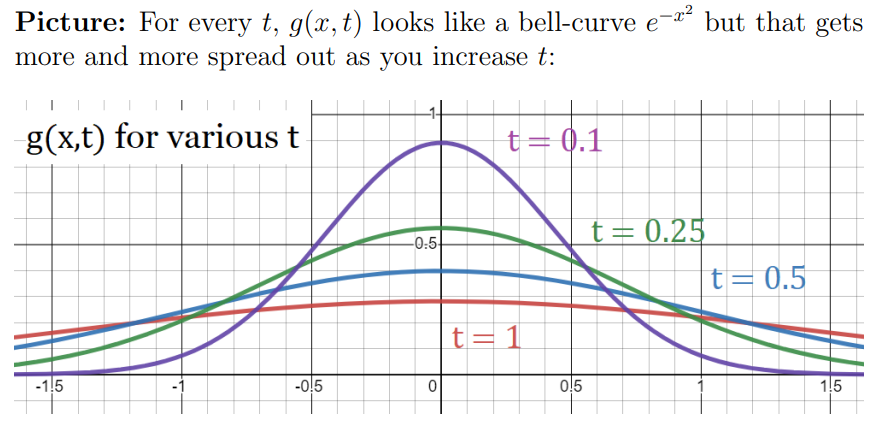
\includegraphics[width=0.8\textwidth]{Images/heat kernel.png}

Note that as $t \to 0^+$, $g(x, t)$ is the Dirac delta at $x = 0$

\subsection*{Part V - Convolution Intuition}
\textbf{Example:} What is the coefficient of $x^2$ in 
\[(x^2 + 2x + 3)(2x^2 + 4x + 1)\]

Generally, the coeff of $x^2$ in $(a_2x^2 + a_1x + a_0)(b_2x^2+ b_1x + b_2)$ is 
\[C_2 = a_0 b_2 + a_1 b_1 + a_2 b_0\] 
and more generally, the coefficient of $x^k$ in $(a_nx^n + ... a_0)(b_nx^n + ... + b_0)$ is 
\[C_k = \sum_{i=0}^k a_i b_{k-1}\]

Note the parallel to 
\[(f \star g)(x) = \int_{-\infty}^\infty f(y)\, g(x -y) \; dy\]

\section*{Lecture 9, Feb 13: Heat Equation Properties}
\subsection*{Part I - Heat Equation Example}
\textbf{Example 1:} Solve 
\[\begin{cases}
    u_t = Du_{xx}\\
    u(x, 0) = e^{-x}
\end{cases}\]

\textbf{Solution:}
\[u(x, t) = \frac{1}{\sqrt4\pi D t} \int_{-\infty}^\infty e^{-\frac{(x - y)^2}{4Dt}} e^{-y} \; dy\]
Looking at the exponent:
\[\frac{-(x-y)^2}{4Dt} - y = -\frac{(x-y)^2 + 4Dty}{4Dt}\]
Expand the numerator:
\[ = -\frac{x^2 - 2xy - y^2 + 4Dty}{4Dt}\]
Note the numerator is a quadratic in y:
\begin{align*}
    y^2 + (4Dt - 2x)y + x^2 &= (y + 2Dt - x)^2 - (2Dt - x)^2 + x^2\\
    &= (y + 2Dt - x)^2 - 4D^2t^2 + 4Dtx - x^2 + x^2\\
    &= (y + 2Dt - x)^2 + 4Dt(x - Dt)
\end{align*}
So the full numerator is 
\[\frac{-(x-y)^2}{4Dt} = -\left(\frac{(y + 2Dt - x)^2 + 4Dt(x - Dt)}{4Dt}\right) = -\left(\frac{(y+2Dt-x)^2}{4Dt}+ (x - Dt)\right)\]
Substituting back in, 
\begin{align*}
    u(x, t) &= \frac{1}{\sqrt4\pi D t} \int_{-\infty}^\infty e^{-\left(\frac{(y+2Dt-x)^2}{4Dt}+ (x - Dt)\right)} \; dy\\
    &= \frac{e^{Dt - x}}{\sqrt4\pi D t}\int_{-\infty}^\infty e^{-frac{(y+2Dt-x)^2}{4Dt}} \; dy\\
    &= \frac{e^{Dt - x}}{\sqrt4\pi D t}\int_{-\infty}^\infty e^{-\left(\frac{y+2Dt-x}{\sqrt{4Dt}}\right)^2} \; dy\\
\end{align*}
Now use u-sub with 
\[p = \frac{y+2Dt-x}{\sqrt{4Dt}}\]
so 
\[dp = \frac{dy}{\sqrt{4Dt}} \implies dy = \sqrt{4Dt} \; dp\]
\[u(x, t) = \frac{e^{Dt - x}}{\sqrt{4\pi D t}}\int_{-\infty}^\infty e^{-p^2} \sqrt{4Dt}\; dp = \frac{e^{Dt - x}}{\sqrt{\pi}} \int_{-\infty}^\infty e^{-p^2}\; dp\]
\[\boxed{u(x, t) = e^{Dt- x}}\]

\subsection*{Part II - Infinite speed of propagation}
Remember the heat equation solution is:
\[u(x, t) = \frac{1}{\sqrt4\pi D t} \int_{-\infty}^\infty e^{-\frac{(x - y)^2}{4Dt}} f(y) \; dy\]
with an initial condition $u(x, 0) = f(x)$

\textbf{Property 1:} If $f \geq 0$ is positive somewhere and continuous, then $u(x, t)$ is positive everywhere. 

This means that heat propagates at infinite speed because heat at one place affects heat everywhere else instantly. Note that the transport equation implies a finite speed of propagation.

\textbf{Why?} 
Suppose $f(x_0) > 0$ for some $x_0$. Then because f is continuous it is actually positive for all x in an interval around $x_0$
Also 
\[u(x, t) = \frac{1}{\sqrt4\pi D t} \int_{-\infty}^\infty e^{-\frac{(x - y)^2}{4Dt}} f(y) \; dy\]
and we know the integrand is non-negative so we have 
\[\frac{1}{\sqrt4\pi D t} \int_{-\infty}^\infty e^{-\frac{(x - y)^2}{4Dt}} f(y) \; dy \geq \frac{1}{\sqrt4\pi D t} \int_{a}^b e^{-\frac{(x - y)^2}{4Dt}} f(y) \; dy\]
But the integrand of the second is also positive so 
\[u(x, t) > 0\] 

\subsection*{Part III  - Smoothness}
\textbf{Property 2:} $u(x, t)$ is infinitely differentiable (for $t >0$) even if $f(x)$ might not be 

\textbf{Why?}
All the derivatives fall of $\exp(-\frac{(x-y)^2}{4Dt})$ and not on f:
\[\frac{d}{dx} u(x, t) = \frac{d}{dx} \frac{1}{\sqrt4\pi D t} \int_{-\infty}^\infty e^{-\frac{(x - y)^2}{4Dt}} f(y) \; dy = \frac{1}{\sqrt4\pi D t} \int_{-\infty}^\infty \frac{d}{dx} e^{-\frac{(x - y)^2}{4Dt}} f(y) \; dy\]
But the term 
\[e^{-\frac{(x - y)^2}{4Dt}}\]
is infinitely differentiable and 
\[\frac{d}{dt}u(x, t) = Du_{xx}\]
but $u_{xx}$ is also smooth 

\subsection*{Part IV - Irreversibility}
\textbf{Property 3:} The heat equation is irreversible ($u(x, 0)$ cannot be determined from $u(x, 1)$)

\textbf{Why?}
"something something entropy"

Suppose $u(x, 1) = |x|$ but by smoothness, $u(x, t)$ must be smooth for all t so $|x|$ must be smooth but this is a contradiction

\section*{Lecture 10, Feb 15: Inverse Fourier Transform}
\subsection*{Part I - Long-time behavior of the heat kernel}
\[u(x, t) = \frac{1}{\sqrt4\pi D t} \int_{-\infty}^\infty e^{-\frac{(x - y)^2}{4Dt}} f(y) \; dy\]

\textbf{Property 4:} 
\[\lim_{t \to \infty} u(x, t) = 0\]
"heat dissipates over time"

\textbf{Why?}
\begin{align*}
    |u(x, t)| &= \left|\frac{1}{\sqrt4\pi D t} \int_{-\infty}^\infty e^{-\frac{(x - y)^2}{4Dt}} f(y) \; dy\right|\\
    &\leq \frac{1}{\sqrt4\pi D t} \int_{-\infty}^\infty |f(y)| \underbrace{e^{-\frac{(x - y)^2}{4Dt}}}_{\leq 1} \; dy\\
    &\leq \frac{1}{\sqrt4\pi D t} \int_{-\infty}^\infty |f(y)| \; dy\\
    &= C \overset{t \to \infty}{\longrightarrow} 0
\end{align*}

\subsection*{Part II - Boundedness}
"u(x, t) does not blow up"

\textbf{Property 5: } If $|f(x) \leq M$ for some M (and all x) then for all x and t we have 
\[|u(x, t) \leq M\]

\textbf{Why?}
\begin{align*}
    |u(x, t)| &= \left|\frac{1}{\sqrt4\pi D t} \int_{-\infty}^\infty e^{-\frac{(x - y)^2}{4Dt}} f(y) \; dy\right|\\
    &\leq \frac{1}{\sqrt4\pi D t} \int_{-\infty}^\infty \underbrace{|f(y)|}_{\leq M} e^{-\frac{(x - y)^2}{4Dt}}\; dy\\
    &\leq \frac{M}{\sqrt4\pi Dt} \int_{-\infty}^\infty e^{-\left(\frac{y - x}{\sqrt{4\pi Dt}}\right)^2}\; dy \quad u = \frac{y - x}{\sqrt{4Dt}} \implies du = \frac{dy}{\sqrt{4Dt}}\\
    &= \frac{M}{\sqrt4\pi Dt} \int_{-\infty}^\infty e^{-u^2}\sqrt{4Dt}\; dy 
    &= \frac{M}{\sqrt4\pi Dt} \sqrt{4Dt} \sqrt{\pi}\\
    &= M
\end{align*}

\subsection*{Part III - Conservation of Mass}
"The area under the curve of u -- no matter its shape -- is always the same"

\[\int_{-\infty}^\infty u(x, t)\; dx =\int_{-\infty}^\infty f(x) \; dx \]

\textbf{Why?}

\emph{Lemma:} 
\[\lim_{x \to \pm \infty} u_x(x, t) = 0\]

Then,
\[u_t = Du_{xx}\]
\[\int_{-\infty}^\infty u_t(x, t)\; dx = \int_{-\infty}^\infty Du_{xx}(x, t)\; dx\]
and by FTC 
\[\frac{d}{dt}\int_{-\infty}^\infty u(x, t) \; dx = D\left[u_x(xm t)\right]_{-\infty}^\infty\]
Thus by the lemma,
\[\frac{d}{dt}\int_{-\infty}^\infty u(x, t) \; dx = D(0- 0) = 0\]
So the integral is constant with respect to time:
\[\int_{-\infty}^\infty u(x, t) \; dx = \int_{-\infty}^\infty u(x, 0) \; dx =\int_{-\infty}^\infty f(x) \; dx\]

\subsection*{Part IV - Inverse Fourier Transform}
Note that for the heat equation, we were very lucky to be able to write the Gaussian as a fourier transform
\[e^{-D\kappa^2t} = \F\left(\frac{1}{\sqrt{4\pi Dt}}e^{-\frac{x^2}{4Dt}}\right)\]
\textbf{But what do we do in general?}

Example: Solve 
\[\begin{cases}
    u_t = -u_{xxxx}\\
    u(x, 0) = f(x)
\end{cases}\]

Solution:
\begin{enumerate}
    \item Fourier transform it
    \[\F\left(u_t\right) = \F\left(-u_{xxxx}\right)\]
    \[\frac{d}{dt} \hat{u} = -(-i\kappa)^4 \hat{u} = -\kappa^4 \hat{u}\]
    \item Solve the ODE 
    \[\hat{u} = u(x, 0)e^{-\kappa^4t} = \hat{f}(\kappa) e^{-\kappa^4t} \]
    \item Write the exponential term as a fourier transform 
    
    \textbf{Definition:} \emph{Inverse Fourier Transform}
    \[\boxed{\check{f}(x) = \mathcal{F}^{-1}(x) = \frac{1}{2\pi} \int_{-\infty}^\infty f(\kappa) e^{-i\kappa x}\; d\kappa}\]

    So in this example, 
    \[e^{-\kappa^4t} = \hat{g}(\kappa) \quad g(x, t) = \mathcal{F}^{-1}\left(e^{-\kappa^4 t}\right) = \frac{1}{2\pi} \int_{-\infty}^\infty e^{-\kappa^4 t} e^{-i\kappa x}\; d\kappa\]

    \item Convolution 
    \item 
    So now we have 
    \begin{align*}
        \hat{u}(\kappa, t) &= \hat{f}(\kappa)e^{-\kappa^4 t}\\
        &= \hat{f}(\kappa) \hat{g}(\kappa, t)\\
        &= \F\left(f \star g\right)(\kappa, t)
    \end{align*}
    Therefore, 
    \[\boxed{\begin{cases}
        u(x, t) = \int_{-\infty}^\infty f(y) g(x - y)\; dy\\
        \text{where} \quad g(x, t) = \frac{1}{2\pi} \int_{-\infty}^\infty e^{-\kappa^4 t} e^{-i\kappa x}\; d\kappa
    \end{cases}}\]
\end{enumerate}

\section*{Lecture 11, Feb 17: Wave Equation Derivation}
\subsection*{Part I - The Wave Equation}
\[u_{tt} = c^2 u_{xx}\]
where $u = u(x, t)$ gives the displacement of a vibrating string at position x and time t and c is a constant giving the speed of the wave  

Note: despite the only difference between this and the heat equation is an extra time derivative, the derivation and solution will be \emph{completely} different

\subsection*{Part II - Derivation}
\begin{enumerate}
    \item Setting: start with a thin string of infinite length and consider a minute sub-piece from $x$ to $x + \Delta x$
    
    \textbf{Assumption:} points on the string only move vertically

    \item By Newton's second law of motion,
    \[F = ma\] 
    By the assumption above and the definition of u, the displacement vector is 
    \[s(x, t) = \brak{0, u(x, t)}\]
    Therefore, acceleration is 
    \[a(x, t) = s_{tt}(x, t) = \brak{0, u_{tt}}\]

    \textbf{Assumption:} the string has constant density $\rho$ 
    
    Then, the mass of the string is density times length (which can be taken by assuming the length is the hypotenuse of a right triangle with legs $\Delta x$ and $\Delta u$). Thus, 
    \[m = \rho \sqrt{(\Delta x)^2 + (\Delta u)^2}\]
    So,
    \[F = ma = \brak{0, \rho \sqrt{(\Delta x)^2 + (\Delta u)^2}}u_{tt}\]

    \item Study of the Force: 
    \textbf{Assumption: The only force acting on the string is the tension}
    So if $T(x, t)$ is the magnitude of the tension vector and $\theta(x, t)$ is the angle of the tension vector:

    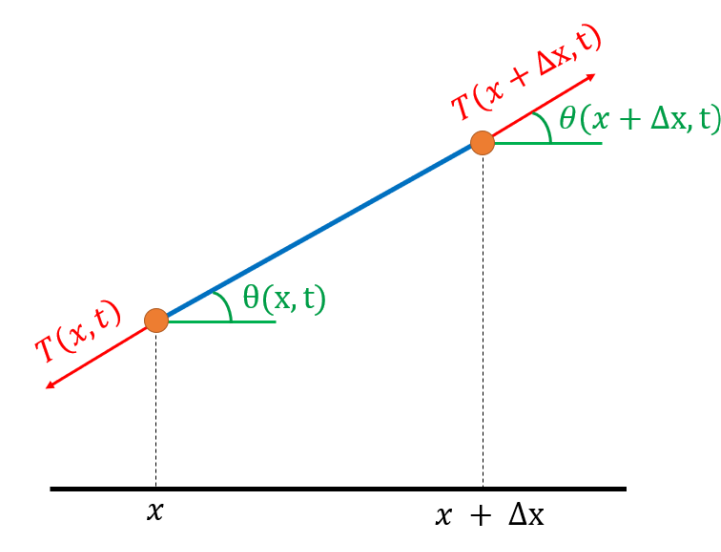
\includegraphics[width=0.8\textwidth]{Images/force.png}

    Then from trig, we can calculate the tension force via components of the resultant:
    \[\begin{cases}
        x = T(x, t) \cos(\theta(x, t))\\
        y = T(x, t) \sin(\theta(x, t))\\ 
    \end{cases} \Longrightarrow -\brak{T\cos(\theta), T\sin(\theta)}(x, t)\]
    Note: the minus comes from T pointing the opposite direction of the string

    Then in the same way, the force at $(x + \Delta x)$ is 
    \[\brak{T\cos(\theta), T\sin(\theta)}(x + \Delta x, t)\]

    so the net force is 
    \[F(x, t) = \brak{T\cos(\theta), T\sin(\theta)}(x + \Delta x, t) - \brak{T\cos(\theta), T\sin(\theta)}(x, t)\]

    \item Then using $F = ma$ and comparing the components, 
    \[\begin{cases}
        T\cos(\theta)(x + \Delta x, t) - T\cos(\theta)(x, t) = 0\\
        T\sin(\theta)(x + \Delta x, t) - T\sin(\theta)(x, t) = \rho \sqrt{(\Delta x)^2 + (\Delta u)^2} u_{tt}(x, t)
    \end{cases}\]
    Note, however, that both these LHS look like derivatives. 
    Starting with the cos terms,
    \[(T\cos(\theta))_x = 0\]
    so $T(x, t)\cos(\theta(x, t))$ is constant in x. 
    But $|\theta(x, t)| << 1$ so $\cos(\theta(x, t)) \approx 1$ and 
    \[T(x, t) \cos(\theta(x, t)) = T(x, t)\]
    which is constant in x so $T(x, t) = T(t)$ 

    \textbf{Assumption:} Tension is also constant in time $T(t) = T$

    Then the sin terms, 
    \begin{align*}
        (T\sin(\theta))_x &= \rho u_{tt} \left(\frac{\sqrt{(\Delta x)^2 + (\Delta u)^2}}{\Delta x}\right)\\
        &= \rho u_{tt} \sqrt{\frac{(\Delta x)^2 + (\Delta u)^2}{\Delta x}} \\
        &= \rho u_{tt}  \sqrt{1 + \left(\frac{\Delta u}{\Delta x}\right)^2} \\
        &= \rho u_{tt} \sqrt{1 + (u_x)^2}
    \end{align*}

    \textbf{Assumption:} if the displacements $\Delta u/\Delta x$ are small, then 
    \[\theta(x, t) = \tan^{-1}\frac{\Delta u}{\Delta x}\]
    is small, proving the inequality above. 

    Then, as $\Delta x \to 0$, $|u_x| << 1$ so 
    \[\sqrt{1 + (u_x)^2} \approx 1\]
    and 
    \[(T\sin(\theta))_x = \rho u_{tt}\]
    but 
    \[\sin \theta  = \tan \theta \cos \theta = \frac{\Delta u}{\Delta x} \cos \theta \to u_x\]
    so 
    \[(Tu_x)_x = Tu_{xx} \quad (\text{assuming T is constant})\] 
    and at last, 
    \[Tu_{xx} = \rho u_{tt} \longrightarrow u_{tt} = \frac{T}{\rho}u_{xx}\]
    Set, $c = \sqrt{T / \rho} > 0$ and 
    \[\boxed{u_{tt} = c^2 u_{xx}}\]
\end{enumerate} 

\section*{Lecture 12, Feb 22: Wave Equation Solution}
\textbf{Goal:} Solve $u_{tt} = c^2 u_{xx}$
\subsection*{Part I - Factoring Method}
But this kind of looks like 
\[t^2 - c^2 x^2 = (t - cx)(t + cx)\]

\textbf{Definition:} Differential operator
\[\frac{\partial}{\partial t} u = u_t\]
\[\left(\frac{\partial}{\partial t}\right)^2 u = u_{tt}\]

Using this operator we can more rigorously "factor" the PDE.

\begin{enumerate}
    \item Apply the differential operator 
    \begin{align*}
        u_{tt} - c^2 u_{xx} &= \left[\left(\frac{\partial}{\partial t}\right)^2 - c^2 \left(\frac{\partial}{\partial x}\right)^2\right]u\\
        &= \left(\frac{\partial}{\partial t} - c \frac{\partial}{\partial x}\right)\left(\frac{\partial}{\partial t} + c \frac{\partial}{\partial x}\right)
    \end{align*}
    \item Solve the equation 
    \[u_{tt} - c^2 u_{xx} = 0\]
    \[\left(\frac{\partial}{\partial t} - c \frac{\partial}{\partial x}\right)\left(\frac{\partial}{\partial t} + c \frac{\partial}{\partial x}\right) = 0\]
    Let $v = \left(\frac{\partial}{\partial t} + c \frac{\partial}{\partial x}\right)u$ 
    so 
    \[\left(\frac{\partial}{\partial t} - c \frac{\partial}{\partial x}\right)v = 0 \Longrightarrow v_t - cV_x = 0\]
    \item Solve the transport PDE 
    \[v(x, t) = f(x + ct)\]
    \item Solve for u 
    \[v := \left(\frac{\partial}{\partial t} + c \frac{\partial}{\partial x}\right)u = u_t + cu_x\]
    \[u_t + cu_x = f(x + ct)\]
    But this is just an inhomogeneous transport equation! 
    The homogeneous solution is just 
    \[u_0(x, t)= G(x - ct)\]
    And a particular solution can be found using undetermined coefficients. Notice that the RHS is a function of $x +ct$ so we can guess 
    \[u_p = h(x + ct)\]
    so 
    \[(h(x + ct))_t + c(h(x + ct))_x = f(x + ct)\]
    \[ch'(x+ ct) + ch'(x + ct) = f(x + ct)\]
    \[2ch'(x + ct) = f(x + ct) \Longrightarrow h' = \frac{1}{2c}f'\]
    \[h(x + ct) = \frac{1}{2c}F(x + ct)\]
    where $F$ is an antiderivative of $f$
    Thus giving the general solution
    \[u(x, t)= G(x - ct) + \frac{1}{2c}F(x + ct) \]
    \[\boxed{u(x, t) = G(x - ct) + F(x + ct)}\]
\end{enumerate}

\textbf{Interpretation:} A wave is a sum of two functions, one moving to the left at speed c and the other to the right at speed c 

\subsection*{Part II - Coordinate Method}
\begin{enumerate}
    \item Define variables 
    \[\begin{cases}
        \xi  =x - ct \\
        \eta = x + ct
    \end{cases}\]
    \item Chain rule 
    \[u_x = \frac{\partial u}{\partial \xi} \frac{\partial \xi}{\partial x} + \frac{\partial u}{\partial \eta} \frac{\partial \eta}{\partial x} = u_\xi + u_\eta\]
    and 
    \begin{align*}
        u_{xx} = (u_x)_x &= \frac{\partial u_x}{\partial \xi} \frac{\partial \xi}{\partial x} + \frac{\partial u_x}{\partial \eta} \frac{\partial \eta}{\partial x} \\
        &= u_{\xi_\xi} + u_{\eta_\eta} = u_{\xi \xi} + u_{\eta \xi} + u_{\xi \eta} + u_{\eta \eta}\\
        &= u_{\xi \xi} + 2u_{\xi \eta} + u_{\eta \eta}
    \end{align*}
    Similarly, 
    \[u_tt = c^2 (u_{\xi \xi} - 2u_{\xi \eta} + u_{\eta \eta})\]

    \item Plug into wave equation:
    \[u_{tt} = c^2 u_{xx}\]
    \[c^2 (u_{\xi \xi} - 2u_{\xi \eta} + u_{\eta \eta}) = c^2( u_{\xi \xi} + 2u_{\xi \eta} + u_{\eta \eta}) = 4u_{\xi \eta}\]
    \[\boxed{u_{\xi \eta} = 0}\]
\end{enumerate}

\section*{Lecture 13, Feb 24: D'Alembert's Formula}
\subsection*{Part I - Solving the wave equation (continued)}
\[u_{tt} = c^2 u_{xx}\]
Using the coordinate method with the choices 
\[\begin{cases}
    \xi = x - ct\\
    \eta = x + ct
\end{cases}\]
we get the equation 
\[u_{\xi \eta} = 0\]
so
\[u_\xi = f(\xi) \Longrightarrow u = F(\xi) + G(\eta)\]
thus 
\[\boxed{u(x, t) = F(x - ct) + G(x + ct)}\]

\subsection*{Part II - D'Alembert's Formula}
\textbf{Example:}
\[\begin{cases}
    u_{tt} = c^2 u_{xx}\\
    u(x, 0) = \phi(x)\\
    u_t(x, 0) = \psi(x)
\end{cases}\]

\textbf{Solution:}
\begin{enumerate}
    \item General Solution
    \[u(x, t) = F(x - ct) + G(x + ct)\]
    \item Plug in the initial condition
    \[u(x, 0) = \phi(x) = F(x) + G(x)\]
    \item Differentiate with t 
    \[u_t(x, t) = -cF'(x - ct) + cG(x + ct)\]
    \[u_t(x, 0) = \psi(x) = -cF'(x) + cG'(x)\]
    \[-F'(x) + G'(x) = \frac{\psi(x)}{c}\]
    \item Integrate over $[0, x]$
    \[\int_0^x -F'(s) + G'(s) \; ds = \int_0^x \frac{\psi(s)}{c} \; ds\]
    \[-F(x) + G(x) - (-F(0) + G(0)) = \frac{1}{c} \int_0^x \psi(s) \; ds\]
    This gives us the system of equations
    \[\begin{cases}
        -F(x) + G(x) = A + \frac{1}{c} \int_0^x \psi(s) \; ds\\
        F(x) + G(x) = \phi(x)
    \end{cases}\]
    \[\Longrightarrow \begin{cases}
        2G(x) = \phi(x) + A + \frac{1}{c} \int_0^x \psi(s) \; ds\\
        2F(x) = \phi(x) - A - \frac{1}{c} \int_0^x \psi(s) \; ds\\
    \end{cases} \Longrightarrow \begin{cases}
        F(X) = \frac{1}{2}\phi(x) - \frac{A}{2} - \frac{1}{2c}\int_0^x \psi(s) \; ds\\
        G(X) = \frac{1}{2}\phi(x) + \frac{A}{2} + \frac{1}{2c}\int_0^x \psi(s) \; ds\\
    \end{cases}\]
    \item Solution 
    \begin{align*}
        u(x, t) &= F(x - ct) + G(x + ct)\\
        &= (\frac{1}{2}\phi(x - ct) - \frac{A}{2} - \frac{1}{2c}\int_0^{x- ct}\psi(s) \; ds) \\
        &\quad + (\frac{1}{2}\phi(x + ct) \frac{A}{2} + \frac{1}{2c}\int_0^{x + ct} \psi(s) \; ds)\\
        &= \frac{1}{2}(\phi(x - ct) + \phi(x + ct)) + \frac{1}{2c}\left(\int_{x-ct}^0 \psi(s)\; ds + \int_0^{x  +ct} \psi(s) \; ds\right)\\
    \end{align*}

    Which at last gives us d'Alembert's equation to solve the wave equation with initial conditions:
    \[\boxed{u(x, t) = \frac{1}{2}(\phi(x - ct) + \phi(x + ct)) + \frac{1}{2c}\int_{x - ct}^{x + ct} \psi(s)\;ds}\]
\end{enumerate}

\subsection*{Part III  - Example}
\[\begin{cases}
    u_{tt} = u_{xx}\\
    u(x, 0) = 0\\
    u_t(x, 0) = \cos(x)\\
\end{cases} \implies \begin{cases}
    c = 1\\
    \phi(x) = 0\\
    \psi(x) = \cos (x)
\end{cases}\]
Then using D'Alembert's:
\begin{align*}
    u(x, t) &= \frac{1}{2}(\phi(x - ct) + \phi(x + ct)) + \frac{1}{2c}\int_{x - ct}^{x + ct} \psi(s)\;ds\\
    &= \frac{1}{2}(0 + 0) + \frac{1}{2} \int_{x - t}^{x +t}\cos(s)\; ds\\
    &= \frac{1}{2}(\sin(x + t) - \sin(x - t))\\
    &= \frac{1}{2}(\sin x \cos t + \cos x \sin t - \sin x \cos -t - \cos x \sin -t)\\
    &= \frac{1}{2}(2 \cos x \sin t)
\end{align*}
\[\boxed{u(x, t) = \sin(t) \cos(x)}\]
(Or, the wave takes the shape of cos with amplitude sin)

\section{Lecture 14, Feb 27: Midterm Review}
\subsection*{Part I  - First Order PDE}
\[\begin{cases}
    (1 + x^2)u_x + e^y u_y = 0\\
    u(0 ,y) = y^2
\end{cases}\]

\[\nabla u \cdot (1 + x^2, e^y) = 0\]
\[y' = \frac{e^y}{1  +x^2}\]
\[\frac{1}{e^y}\; dy = \frac{1}{1 + x^2}\; dx\]
\[\tan^{-1} x = -e^{-y} + C \implies \tan^{-1}x + e^{-y} = C\]
\[u(x, y) = f(\tan^{-1}(x) + e^{-y})\]
\[u(0, y) = f(\tan^{-1}(0) + e^{-y}) = y^2 = f(e^{-y})\]
\[z := e^{-y} \implies -y = \ln z \implies y = - \ln z\]
\[f(z) = f(e^{-y}) = y^2 = (-\ln(z))^2 = (\ln z)^2\]
\[\boxed{u(x, y) = \ln(\tan^{-1} x + e^{-y})^2}\]

\subsection*{Part II - Coordinate Method}
\[au_x + bu_y + cu = 0\]

Solution:
\[\begin{cases}
    \xi = ax + by\\
    \eta = ay - bx
\end{cases}\]
\[\begin{cases}
    u_x = u_\xi \xi_x + u_\eta \eta_x = au_\xi -bu_\eta\\
    u_y = u_\xi \xi_y + u_\eta \eta_y = bu_\xi + au_\eta
\end{cases}\]
\begin{align*}
    au_x + bu_y + cu &= a(au_\xi -bu_\eta) + b(bu_\xi + au_\eta) + cu\\
    &= a^2u_\xi - abu_\eta + b^2 u_\xi + abu_\eta + cu\\
    &= (a^2 + b^2) u_\xi + cu\\
    &= u_\xi + \frac{c}{a^2 + b^2}u = 0
\end{align*}
\[u = f(\eta)e^{-\frac{c}{a^2 + b^2}\xi}\]
\[\boxed{u(x, y) = f(ay -bx)e^{-\left(\frac{c}{a^2 + b^2}\right)(ax + by)}}\]

\subsection*{Part III - Fourier Transform}
\[\begin{cases}
    au_x + bu_t + cu = 0\\
    u(x, 0) = f(x)
\end{cases}\]

Solution:
\[\F(au_x) + \F(bu_t) + \F(cu) \implies \F(bu_t) = -\F(au_x) -\F(cu)\]
\begin{align*}
    b\frac{d}{dt}\hat{u} &= -a(-i\kappa)\hat{u} - c\hat{u} \\
    \frac{d}{dt}\hat{u} &= \left(\frac{ai\kappa - c}{b}\right)\hat{u} \\
    \hat{u} &= \hat{f}(\kappa)e^{\frac{ai\kappa - c}{b}t}\\
    &= \hat{f}(\kappa)e^{i\kappa\left(\frac{a}{b}\right)t} e^{-\frac{ct}{b}}\\
    &= e^{-\frac{ct}{b}} \F\left(f(x - \frac{a}{b}t)\right)\\
    &= \F\left(e^{-\frac{ct}{b}}f(x - \frac{a}{b}t)\right)
\end{align*}
\[\boxed{u(x, t) = e^{-\frac{ct}{b}}f(x - \frac{a}{b}t)}\]

\subsection*{Part IV - Wave Equation Factoring Method}
\[3u_{tt} + 10u_{xt} + 3u_{xx} = 0\]
Solution:
\[3t^2 + 10xt + 3x^2 \implies \left(x + 3t\right)\left(3x+ t\right)\]
\begin{align*}
    3u_{tt} + 10u_{xt} + 3u_{xx} &= 3\frac{\partial^2}{\partial t^2}+ 10\frac{\partial^2}{\partial x\partial t} + 3\frac{\partial^2}{\partial x^2}\\
    &= \left(\frac{\partial}{\partial x}+ 3\frac{\partial}{\partial t}\right)\left(3\frac{\partial}{\partial x}+ \frac{\partial}{\partial t}\right)u\\
\end{align*}
Let 
\[v = \left(3\frac{\partial}{\partial x}+ \frac{\partial}{\partial t}\right)u\]
so 
\[\left(\frac{\partial}{\partial x}+ 3\frac{\partial}{\partial t}\right)v = 0\]
\[v_x + 3v_t = 0 \implies v = f(x - \frac{t}{3})\]
Then
\[\left(3\frac{\partial}{\partial x}+ \frac{\partial}{\partial t}\right)u = 3u_x + u_t  = f(x - \frac{t}{3})\]

Homogeneous solution:
\[3u_x + u_t = 0 \implies u_0(x, t) = G(x - 3t)\]

Particular solution:
\[f(x - 3t) \implies u_p(x, t) = h(x - \frac{t}{3})\]
\[3(h(x - \frac{t}{3}))_x + (h(x - \frac{t}{3}))_t = f(x - \frac{t}{3})\]
\[\implies h(s) = \frac{3}{8}F(S)\]
\[u_p = \frac{3}{8}F(x - \frac{t}{3})\]
\[u(x, t) = G(x - 3t) + \frac{3}{8}F(x - \frac{t}{3})\]
\[\boxed{u(x, t) = G(x - 3t) + F(x - \frac{t}{3})}\]

\section{Lecture 15, March 3: Energy Methods}
\subsection*{Energy Method for Waves}
\textbf{Example 1: Conservation of Energy}
Suppose u solves the wave equation $u_{tt} = c^2 u_{xx}$. Then the following is constant 
\[E(t) = \frac{1}{2}\int_{-\infty}^\infty (u_t)^2 + c^2(u_x)^2\; dx\]
where $(u_t)^2 = \frac{1}{2}mv^2$ is the kinetic energy and the second term $c^2(u_x)^2$ is the potential energy. Thus, for the wave equation, the total energy is conserved. 

\emph{Method 1:} Calculate $E'(t)$ and show it is 0
This is easier but requires you know E a priori.

\emph{Method 2:} Energy Method
\begin{enumerate}
    \item Start with $u_t = c^2 u_{xx}$
    \textbf{Trick:} Multiply the PDE by a clever function, here by $u_t$
    \[u_{tt}u_t = c^2 u_{xx}u_t\]
    Integrate with respect to x:
    \[\int_{-\infty}^\infty u_{tt}u_t \; dx = c^2 \int_{-\infty}^\infty u_{xx}u_t \; dx\]

    \item Study A 
    From calculus,
    \[y'' y' = \left[\frac{1}{2}(y')^2\right]'\]
    Therefore, 
    \[u_{tt}u_t = \frac{d}{dt}\left[\frac{1}{2}(u_t)^2\right]\]
    so 
    \[A = \int_{-\infty}^\infty u_{tt} u_t \; dx = \frac{d}{dt} \left(\frac{1}{2}\int_{-\infty}^{\infty} (u_t)^2 \; dx\right)\]


    \item Study B 
    \[B = \int_{-\infty}^{\infty} u_{xx}u_t \; dx\]
    Integrate by parts WRT x:
    \begin{align*}
        A &= \int_{-\infty}^{\infty} u_{xx} u_t \; dx\\
        &\overset{\text{IBP}}{=} [u_xu_t]_{-\infty}^\infty - \int_{-\infty}^{\infty} u_x u_{xt} \; dx\\
        &= - \int_{-\infty}^{\infty} u_x u_{xt}\; dx\\
        &= - \int_{-\infty}^{\infty} \frac{d}{dt} \left(\frac{1}{2}(u_x)^2\right)\; dx\\
        &= \frac{d}{dt}\left(-\frac{1}{2}\int_{-\infty}^{\infty} (u_x)^2 \; dx\right)
    \end{align*}

    \item Then $A = c^2 B$ implies 
    \[\frac{d}{dt}\left(\frac{1}{2}\int_{-\infty}^{\infty} (u_t)^2 \; dx\right) = c^2 \frac{d}{dt}\left(-\frac{1}{2}\int_{-\infty}^{\infty} (u_x)^2 \; dx\right)\]
    \[\frac{d}{dt}\left(\frac{1}{2}\int_{-\infty}^{\infty} (u_t)^2 + c^2 (u_x)^2\; dx\right) = 0\]
    \[\frac{d}{dt}E(t) = 0\]
    so E is constant
\end{enumerate}

\textbf{Note:} How do we know which function to multiply the PDE by? It's an art! Here we multiplied by $u_t$ to make a time-derivative appear

\subsection*{Application: Uniqueness}
\textbf{Lemma:}
Suppose $w$ solves the following PDE
\[\begin{cases}
    w_{tt} = c^2 w_{xx}\\
    w(x, 0) = 0\\
    w_t(x, 0)= 0
\end{cases}\] 
Then $w(x, t) = 0$ for all x and t.

\textbf{Why?}
\begin{enumerate}
    \item the energy $E(t)$ is constant so 
    \[E(t) = E(0)\]
    \[\frac{1}{2} \int_{-\infty}^{\infty} (w_t)^2 + c^2 (w_x)^2 \; dx = \frac{1}{2} \int_{-\infty}^{\infty} (w_t(x, 0))^2 + c^2(w_x(x, 0))^2\; dx\]
    By assumption, we have $w_t(x, 0) = 0$ and moreover
    \[w(x, 0) = 0 \implies (w(x, 0))_x = 0 = 0_x \implies w_x(x, 0) = 0\]
    Therefore the above becomes 
    \[\frac{1}{2}\int_{-\infty}^{\infty} (w_t)^2 + c^2(w_x)^2 = 0\]

    \item 
    \textbf{Fact:} if $f \geq 0$ and $\int_{-\infty}^{\infty} f(x)\; dx = 0$ then f must be the zero-function  

    Therefore $(w_t)^2 + c^2(w_x)^2 = 0$ 
    So $w_t = 0$ and $w_x = 0$
    Hence $w(x, t) = C$
    But plugging in $t= 0$ we get $C = w(x, 0) = 0$ and $w(x, t) = 0 \quad \square$

    \textbf{Application:}
    There is at most one solution of 
    \[\begin{cases}
        u_{tt} = c^2 u_{xx}\\
        u(x, 0) = \phi(x)\\
        u_t(x, 0) = \psi(x)
    \end{cases}\]

    \textbf{Proof:}
    Standard trick: suppose there are two solutions u and v and let $w = u - v$. Then we check that w solves 
    \[\begin{cases}
        u_{tt} = c^2 u_{xx}\\
        u(x, 0) = u(x, 0) - v(x, 0) = \phi(x) - \phi(x) = 0\\
        u_t(x, 0) = u_t(x, 0) - v_t(x, 0) = \psi(x) - \psi(x) = 0
    \end{cases}\]
    By the lemma above, we get $w = 0$ so $u-v=0$ so $u=v$
    and thus there is exactly one solution of the above wave equation
\end{enumerate}

\subsection*{Energy Method for Heat}
Suppose we have a finite rod of length l with initial temperature 0 and insulated. 

\textbf{Example 2:} 
Suppose u solves the PDE
\[\begin{cases}
    u_t = Du_{xx}\\
    u(x, 0) = 0\quad \text{Initial}\\
    u(0, t) = 0\quad \text{Endpoint}\\
    u(l, t) = 0\quad \text{Endpoint}
\end{cases}\]
Then $u(x, t) = 0$ for all x and t 

\textbf{Proof:}
\begin{enumerate}
    \item Start with $u_t = Du_{xx}$. Multiply by u 
    \[u_t u = Du_{xx}u\] 
    Integrate with respect to x on $[0, l]$
    \[\int_0^l u_t u \; dx = F \int_0^l u_{xx}u\; dx\]
    \item Study A 
    \[A = \int_0^l \frac{d}{dt}\left(\frac{1}{2}u^2\right) \; dx = \frac{d}{dt} \left(\int_0^l u^2 \; dx\right)\]
    \item Study B
    \[\int_0^l u_{xx} u\; dx = u_x(l, t)u(l, t) - u_x(0, t) - \int_0^l u_x u_x \; dx = -\int_0^l (u_x)^2\;dx\]

    \item So $A = DB$ and 
    \[\frac{d}{dt}\left(\frac{1}{2}\int_0^l u^2 \; dx\right) = -D\int_0^l (u_x)^2 \; dx \leq 0\]
    Then if you define 
    \[E(t) = \frac{1}{2}\int_0^l u^2 \; dx\]
    you have $E'(t) \leq 0$ so the energy is decreasing 

    \textbf{Interpretation:} heat is dissipative. An insulated metal rod generally gets cooler with time

    This also means that 
    \[E(t) \leq E(0)\]
    so 
    \[E(t) = \frac{1}{2}\int_0^l (u(x, t)^2)\; dx \leq E(0) = \frac{1}{2}\int_0^l (u(x, 0))^2\; dx = 0\]

    \item Finale
    But $E(t) \geq 0$ by definition so $0 \leq E(t) \leq E(0) = 0 \implies E(t) = 0$ and 
    \[\frac{1}{2}\int_0^l (u(x, t))^2\; dx = 0\]
    Therefore $(u(x, t))^2 =0$ so $u(x, t) = 0$ for all x and t
\end{enumerate}

\section{Lecture 16, March 6: Heat vs Wave Equations}
\subsection*{Part I - Energy Method Application}
\textbf{Example:}
\[\begin{cases}
    u_t = Du_{xx} + f(x, t)\\
    u(x, 0) = \phi(x)\\
    u(0, t) = g(t)\\
    u(l, t) = h(t)
\end{cases}\]
\textbf{Trick:} $w := u - v$ and via the initial conditions, $w = 0$ so $u = v$ and there is only one solution

\subsection*{Part II - The Infinite Rod}
\textbf{Example:}
\[\begin{cases}
    u_t = Du_{xx}\\
    u(x, 0) = f(x)
\end{cases}\]
has many solutions including $u = f\star g$

\textbf{Note:} we have uniqueness if 
\[|u(x, t)| \leq Ce^{ax^2}\]
for some $C > 0$ and $a > 0$ (meaning the PDE is in the Schwartz class)

\subsection*{Part III - Comparison of Waves and Diffusions}
\begin{center}
    \begin{tabular}{|c | c|}
        \hline\\
        Heat Equation & Wave Equation\\
        $\begin{cases}
            u_t = Du_{xx}\\
            u(x, 0) = f(x)
        \end{cases}$ & $\begin{cases}
            u_{tt} = c^2 u_{xx}\\
            u(x, 0) = \phi(x)\\
            u_t(x, 0) = \psi(x)
        \end{cases}$\\
        \hline
        Existence via Fourier Transform & Existence via Factoring\\
        $u(x, t) = \frac{1}{\sqrt{4\pi Dt}} \int_{-\infty}^\infty e^{-\frac{(x-y)^2}{4Dt}} f(y) \; dy$ & $u(x, t) = \frac{1}{2}(\phi(x - ct) + \phi(x + ct)) + \frac{1}{2c}\int_{x - ct}^{x+ ct} \psi(s) \; ds$\\
        \\
        Uniqueness (given u is Schwartz) & Uniqueness by energy method\\
        \\
        Smooth & Not smooth\\
        (infinite differentiability of heat kernel) &  (initial condition splits but will not smooth)\\
        \\
        Infinite speed of propagation & Finite speed of propagation\\
        \\
        Not reversible & Reversible (if wave travels backwards)\\
        \\
        Goes to zero over time (energy is decaying) & Does not go to zero (energy is conserved)\\
        \hline
    \end{tabular}
\end{center}

\section{Lecture 17, March 8: Separation of Variables I}
This is the most important PDE technique in the course. 

\subsection*{Part I - Boundary Value Problem}
\textbf{Example 1:}
Find all the values of $\lambda$ for which the following ODE has a nonzero solution X 
\[\begin{cases}
    X''(X) = \lambda X(x)\\
    X(0) = 0\\
    X(\pi) = 0
\end{cases}\]

Case 1: $\lambda > 0$ 
Then $\lambda = \omega^2$ for positive $\omega$ and the aux equation is 
\[r^2 = \omega^2 \implies r = \pm \omega\]
so 
\[X(x) = Ae^{\omega x} + Be^{-\omega x}\] 
\[X(0) = A + B = 0 \implies B = -A\]
\[X(x) = Ae^{\omega x} -Ae^{-\omega x}\]
\[X(\pi) = 0 \implies Ae^{\omega \pi} -Ae^{-\omega pi} = 0 \implies 2\pi \omega = 0\]
But then $\lambda = 0$ which contradicts $\lambda >0$ so no nonzero solutions 

Case 2: $\lambda = 0$
Aux: $r^2 = 0 \implies r = 0$
\[X(x) = A + Bx \implies X(0) = A = 0 \implies X(x) = Bx\]
\[X(\pi) = 0 \implies B\pi = 0 \implies B = 0\]
But then 
\[X(x) = 0\]
So there are no nonzero solutions here either 

Case 3: $\lambda < 0$
\[r^2 = \lambda = -\omega^2 \implies r = \pm \omega i\]
\[X(x) = A\cos(\omega x) + B\sin(\omega x)\]
\[X(0) = A = 0 \implies X(x) = B\sin(\omega x)\]
\[X(\pi) = 0 \implies \sin(\omega \pi) = \implies \omega \pi = \pi m \implies \omega = m\]
Where m is any positive integer. So our eigenvalues are
\[\lambda = -m^2 \quad (m = 1, 2, ...)\]
and our eigenfunctions are 
\[X(x) = \sin(mx) \quad (m = 1, 2, ...)\]

\subsection*{Part II - Separation of Variables}
\textbf{Example 2:}
\[\begin{cases}
    u_t = Du_{xx}\\
    u(0, t) = 0\\
    u(\pi, t) = 0\\
    u(x, 0) = x^2
\end{cases}\]
Note that this is the same finite rod problem for which we proved uniqueness via energy methods. Then we just need to find one nonzero solution.

Solution:
\begin{enumerate}
    \item Separation of variables 
    Assume u is the form $u(x, t) = X(x)T(t)$
    Plug into the PDE:
    \[u_t = Du_{xx}\]
    \[(X(x)T(t))_t = D(X(x)T(t))_{xx}\]
    \[X(x)T'(t) = DX''(x)T(t)\]
    \[\frac{T'(t)}{DT(t)} = \frac{X''(x)}{X(x)}\]
    Note: always put extra terms on the T side to keep the X equation simple

    \item Constant 
    Note that 
    \[\left(\frac{X''(x)}{X(x)}\right)_t = 0\]
    and 
    \[\left(\frac{X''(x)}{X(x)}\right)_x = \left(\frac{T'(t)}{DT(t)}\right)_x = 0\]
    so 
    \[\frac{X''(x)}{X(x)} = \frac{T'(t)}{DT(t)} = \text{Constant} = \lambda\]
    Then 
    \begin{align*}
        X''(x) = \lambda X(x)\\
        T'(t) = D\lambda T(t)
    \end{align*}
    and instead of a PDE we have two ODEs!

    Focusing on the X equation, 
    \[X''(x) = \lambda X(x)\]
    we can use the boundary conditions
    \[u(0, t) = 0 \overset{u=XT}{\Longleftarrow} X(0)T(t)= 0 \implies X(0) =0\]
    (you can cancel the T because fo $T= 0$ the problem is not interesting)
    \[u(\pi, t) =0 \implies X(pi) = 0\]

    So 
    \[\begin{cases}
        X''(x) &= \lambda X(x)\\
        X(0) &= 0\\
        X(\pi) &= 0
    \end{cases}\]
    which is the same ODE from part I! 

    \[\begin{cases}
        \lambda = -m^2 \quad (m = 1, 2, ...)\\
        X(x) = \sin(mx) \quad (m = 1, 2, ...)
    \end{cases}\]

    \item T equation 
    \[\begin{cases}
        \frac{T'}{DT} = \lambda = -m^2\\
        T' = -m^2DT\\
        T(t) = e^{-m^2 Dt}
    \end{cases}\]

    Conclusion: For every $m = 1, 2, ...$ 
    \[u(x, t) = X(x)T(t) = \sin(mx)e^{-m^2Dt}\]
    is a solution to the PDE 

    \item Linearity
    Since the PDE is linear, any linear combo of the above solution is also a solution!
    \[u(x, t) = \sum_{m=1}^\infty A_m \sin(mx)e^{-m^2Dt}\]

    \item Initial Condition 
    \[u(x, 0) = \sum_{m=1}^\infty A_m \sin(mx) = x^2\]

    \textbf{Question:} How do you find $A_m$ (can you write $x^2$ as a linear combo of sines?)
\end{enumerate}

\subsection*{Part III - Easier Problem}
\[\begin{cases}
    u_t = Du_{xx}\\
    u(0, t) = 0\\
    u(\pi, t) = 0\\
    u(x, 0) = 3\sin(2x) + 4\sin(3x)
\end{cases}\]

The steps above give 
\[u(x, t) = \sum_{ m=1}^\infty A_m \sin(mx)e^{-m^2Dt}\] 
so 
\[u(x, 0) = \sum_{ m=1}^\infty A_m \sin(mx) = 3\sin(2x) + 4\sin(3x)\]
and 
\[\boxed{u(x, t) = 3\sin(2x)e^{-4Dt} + 4\sin(3x)e^{-9Dt}}\]

\textbf{Interpretation:} Initially, the solution starts out as the sum of sines but eventually dies down as the exponential terms go to 0

\section*{Lecture 18, March 10: Separation of Variables II}
\subsection*{Part I - Setting}
\textbf{Example 1:}
\[\begin{cases}
    u_{tt} = c^2 u_{xx} \quad 0 < x < 1\\
    u(0, t) = 0\\
    u(1, t) = 0\\
    u(x, 0) = x^2\\
    u_t(x, 0) = e^x
\end{cases}\] 

Note that you cannot use d'Alembert's formula because the bounds are not $-\infty < x < \infty$

\subsection*{Part II - Separation of variables}
Assume that 
\[u(x, t) = X(x) T(t)\]
Then plug this in 
\[(X(x)T(t))_{tt} = c^2((X(x)T(t))_{xx})\]
\[XT'' = c^2X''T\]
\[\frac{X''}{X} =  \frac{T''}{c^2T}\]
Note that 
\[\left(\frac{X''}{X}\right)_t = 0\]
\[\left(\frac{X''}{X}\right)_x = \left(\frac{T''}{c^2T}\right)_x = 0\]
so 
\[\frac{X''}{X} =  \frac{T''}{c^2T} = \lambda\]
with $\lambda$ constant. Then 
\begin{align*}
    X'' = \lambda X\\
    T'' = c^2\lambda T
\end{align*}
Using the boundary conditions
\[u(0, t) = 0 \implies X(0)T(t)= 0 \implies X(0) = 0\]
\[u(1, t) = 0 \implies X(1)T(t)= 0 \implies X(1) = 0\]

Then looking at the X ODE:
\[\begin{cases}
    X'' = \lambda X\\
    X(0) = 0\\
    X(1) = 0
\end{cases}\]
\[r^2 = \lambda \implies r = \pm \omega\]
Case $\lambda > 0$:
\[X = Ae^{\omega x} + Be^{-\omega x}\]
Initial conditions show no nonzero solutions

Case $\lambda = 0$:
\[X(x) = A + Bx \longrightarrow X(0) =A  =0  \longrightarrow X(x) = 0\]

Case $\lambda < 0$:
\[r^2 = \lambda = - \omega^2 \implies r = \pm \omega i\]
\[X(x) = A \cos(\omega X) + B\sin(\omega X)\]
\[X(0) = A = 0 \implies X(x) = B\sin(\omega x)\]
\[X(1) = B\sin(\omega) = 0\]
\[\sin(\omega) = 0 \implies \omega = \pi m \quad (m = 1, 2, ...)\]
\begin{align*}
    \lambda &= -\omega^2 = -(\pi m)^2 \quad (eigenvalues)\\
    X(x) &= \sin(\pi m x) \quad (eigenfunction)
\end{align*}

Now going all the way back to the T equation:
\[T'' = c^2\lambda T\]
\[\frac{T''}{c^2T} = \lambda = -(\pi m)^2\]
\[T'' = -(\pi m)^2 c^2 T\]
\[T'' = -(\pi m c)^2T \]
\[T'' -(\pi m c)^2T =0\]
Auxiliary:
\[r^2 - (\pi m c)^2 = 0\]
\[r = \pm \pi m ci\]
\[T = A\cos(\pi m ct) + B\sin(\pi mct)\]

Conclusion:
\[u(x, t) = X(x)T(t) = (A\cos(\pi m ct) + B\sin(\pi mct)) \sin(\pi m x)\]

General solution via linearity:
\[\boxed{u(x, t) = \sum_{m=1}^\infty (A_m\cos(\pi m ct) + B_m\sin(\pi mct)) \sin(\pi m x)}\]
 
Initial conditions:
\[u(x, 0) = \sum_{m=1}^\infty (A_m\cos(0) + B_m\sin(0)) \sin(\pi m x) = \sum_{m=1}^\infty A_m \sin(\pi m x) = x^2\]
The question of representing an arbitrary function as a sum of sin waves deals with Fourier series and will come up later.
\[u_t = \sum_{m=1}^\infty (-A_m\pi m c \sin(\pi m ct) + B_m \pi m c \cos(\pi mct)) \sin(\pi mx)\]
\[u_t(x, 0 ) = \sum_{m=1}^\infty B_m \pi mc\sin(\pi mx) = e^x\]

\subsection*{Part III - Easier initial conditions}
\textbf{Example 2:}
\[\begin{cases}
    u_{tt} = c^2 u_{xx} \quad 0 < x < 1\\
    u(0, t) = 0\\
    u(1, t) = 0\\
    u(x, 0) = 2\sin(2\pi x) + 3\sin(3\pi x)\\
    u_t(x, 0) = 4\sin(2\pi x)
\end{cases}\] 

General solution:
\[u(x, t) = \sum_{m=1}^\infty (A_m\cos(\pi m ct) + B_m\sin(\pi mct)) \sin(\pi m x)\]

Initials:
\begin{align*}
    u(x, 0) &= \sum_{m=1}^\infty A_m \sin(\pi m x)\\
    &= A_1\sin(\pi x) + A_2\sin(2\pi x) + A_3\sin(3\pi x) + ...\\
    &= 0\sin(\pi x) + 1\sin(2\pi x) + 3\sin(3\pi x) + 0\sin(4\pi x)+ ...\\
\end{align*}
therefore, 
\[A_1 = 0 \quad A_2 = 1 \quad A_3 = 3 \quad A_m = 0 \; (m \geq 4)\]
And from the other initial condition
\[u_t(x, 0) = \sum_{m=1}^\infty (\pi mc)B_m\sin(\pi mx) = \pi cB_1 \sin(\pi x) + 2\pi cB_2\sin(2\pi x) + 3\pi cB_3\sin(3\pi x) = 4\sin(2\pi x)\]
so 
\[B_1 = 0 \quad B_2 = \frac{2}{\pi c} \quad B_m = 0 \; (m \geq 3)\]
and 
\begin{align*}
    u(x, t) &= \sum_{m=1}^\infty =(A_m\cos(\pi m ct) + B_m\sin(\pi mct)) \sin(\pi m x) \\
    &= (A_2\cos(2\pi ct) + B_2\sin(2\pi ct)) \sin(2\pi x) + (A_3\cos(3\pi ct) + B_3\sin(3\pi ct)) \sin(3\pi x)
\end{align*}
At long last,
\[\boxed{u(x, t) = \left(\cos(2\pi ct) + \frac{2}{\pi c}\right)\sin(2\pi x) + (2\cos(3\pi ct))\sin(3\pi x)}\]

\section*{Lecture 20, March 13: Separation of Variables III}
\subsection*{Part I - Setting}
Heat equation but assuming velocity at the endpoints is 0 (``rate in = rate out'')
\[\begin{cases}
    u_t = Du_{xx}\\
    u_x(0, t) = 0\\
    u_x(\pi, t) = 0\\
    u(x, 0) = x^2
\end{cases}\]

\subsection*{Part II - Separation of variables}
Suppose $u(x, t) = X(x)T(t)$
Plug in 
\[(X(x)T(t))_t = D(X(x)T(t))_{xx} \]
\[XT' = DX''T\]
\[\frac{T'}{DT} = \frac{X''}{X} = \lambda\]
\[\begin{cases}
    X'' = \lambda X\\
    T' = \lambda DT
\end{cases}\]

X boundary conditions:
\begin{align*}
    u = XT\\
    u_x = X'T\\
    u_x(0, t) = 0 \implies X'(0) = 0\\
    u_x(\pi, t) = 0 \implies X'(\pi) = 0
\end{align*}
So 
\[\begin{cases}
    X'' = \lambda X\\
    X'(0) = 0\\
    X'(\pi) = 0
\end{cases}\]

Boundary value problem:
Case 1 $\lambda > 0$:
\[r^2 = \lambda = \omega^2 \implies r = \pm \omega\]
\[X = Ae^{\omega x} + Be^{-\omega x}\]
\[X'(0) = A - B = 0 \implies A = B\]
\[X = Ae^{\omega x} + Ae^{-\omega x}\]
\[X'(pi) = 0 \implies \omega \pi = -\omega \pi \implies \omega = 0\]
No nonzero solutions

Case 2 $\lambda = 0$
\[r^2 = 0 \implies X = A + Bx\]
\[X'(0) = 0 \implies B = 0\implies X = A\]
So $\lambda = 0$ is an eigenvalue with eigenfunction $X(x) = A$

Case $\lambda < 0$:
\[r^2 = \lambda = -\omega^2 \implies r = \pm \omega i\]
\[X = A\cos(\omega x) + B\sin(\omega x)\]
\[X'(0) = B\omega = 0 \implies X = A\cos(\omega x)\]
\[X'(\pi) = 0 \implies \sin(\omega \pi)=0 \implies \omega = m\]
\[\lambda = -\omega^2 = -m^2\]
So with the above case, the eigenvalues are 
\[\lambda = -m^2 \quad (m = 0, 1, 2, ...)\]
and the eigenfunctions are 
\[X(x) = \cos(mx) \quad (m = 0, 1, 2,...)\]

Back to the T equation:
\[\frac{T'}{DT} = \lambda = -m^2\]
\[T' = -m^2DT\]
\[T(t) = e^{-m^2Dt}\]

Conclusion: 
for every $m = 0, 1, 2, ...\quad $ the following solves the PDE:
\[u(x, t) = X(x)T(t) = e^{-m^2Dt}\cos(mx)\]

Taking linear combinations we get 
\[u(x, t) = \sum_{m=0^\infty}A_m e^{-m^2Dt}\cos(mx)\]
So with the initial condition 
\[x^2 = \sum_{m=0}^\infty A_m \cos(mx)\]

\subsection*{Part III - Inhomogeneous Problems}
\textbf{Example 2:}
\[\begin{cases}
    u_t = Du_{xx}\\
    u(0, t) = 7\\
    u(\pi, t) = 7\\
    u(x, 0) = x^2
\end{cases}\]

Trick: Let $v(x, t) = u(x, t) - 7$
Then 
\[v_t = (u - 7)_t = u_{tt} = Du_{xx} = D(v + 7)_{xx} = Dv_{xx}\]
\begin{align*}
    v(0, t) &= u(0, t) - 7 = 0\\
    v(\pi, t) &= u(\pi, t) - 7 = 0\\
    v(x, 0) &= u(x, 0) - 7= x^2 - 7
\end{align*}
Then solve the above system for v using separation of variables and use 
\[u(x, t) = v(x, t) + 7\]
to solve for u

\textbf{Example 3:}
\[\begin{cases}
    u_t = Du_{xx}\\
    u_x(0, t) = 7\\
    u_x(\pi, t) = 7\\
    u(x, 0) = x^2
\end{cases}\]

Trick: Use $v(x, t) = u(x, t) - 7x$
Then 
\[v_t = (u - 7x)_t = u_t = Du_{xx} = D(v + 7x)_{xx} = Dv_{xx}\]
\begin{align*}
    v_t &= Dv_{xx}\\
    v_x(0, t) &= u_x(0, t) - 7 = 0\\
    v_x(\pi, t) &= u_x(\pi, t) - 7 = 0\\
    v(x, 0) &= u(x, 0) - 7x = x^2 - 7x
\end{align*}
Solve for v using separation of variables and use 
\[u(x, t) = v(x, t) + 7x\]

\textbf{Example 4:}
\[\begin{cases}
    u_t = Du_{xx}\\
    u(0, t) = 1\\
    u(\pi, t) = 3\\
    u(x, 0) = x^2
\end{cases}\]
Let $v(x, t) = u(x, t) - f(x)$
Where f is a linear function such that $f(0) = 1$ and $f(\pi) = 3$
Then 
\[f(x) = \left(\frac{3 - 1}{\pi - 0}\right)(x -0) + 1 = \frac{2}{\pi}x + 1\]
\[v(x, t) = u(x, t) - frac{2}{\pi}x - 1\]
\[v_t = (u - f(x))_t = u_t = D(v + f(x))_{xx} = Dv_{xx}\]
Here we used $f''(x)$ since f is linear 
\begin{align*}
    v(0, t) &= u(0, t) - f(0) = 1 - 1=0\\
    v(\pi, t) &= u(\pi, t) - f(\pi) = 3 - 3=0\\
    v(x, 0) &= u(x, 0) - f(x) = x^2 - \frac{2}{\pi}x- 1\\
\end{align*}
Then solve 
\[\begin{cases}
    v_t = Dv_{xx}\\
    v(0, t) = 0\\
    v(\pi, t) = 0\\
    v(x, 0) = x^2 - \frac{2}{\pi}x - 1
\end{cases}\]
Then 
\[u(x, t) = v(x, t) + f(x) = v(x, t) + \frac{2}{\pi}x + 1\]
Note: we could in theory also solve the case where $u_x(0, t) = 1$ and $u_x(\pi, t) = 3$ by subtracting a function whose \emph{derivative} is $\frac{2}{\pi}x + 1$ except you would get an inhomogeneous wave equation for v

\section*{Lecture 21, March 15: Fourier Series (I)}
\subsection*{Part I - Prelude}
\textbf{Goal:} given a function $f(x)$ on $(0, \pi)$ find $A_m$ such that 
\[f(x) = \sum_{m=1}^\infty A_m \sin(mx)\]
This is known as a Fourier sine series and is similar to a Taylor series 

\subsection*{Part II - Orthogonality}
\textbf{Definition:} Let $u, \; v, \; w$ be vectors. Then $u$ and $v$ are orthogonal if 
\[u \cdot v = 0\]
and $\{u, v , w\}$ is orthogonal if any two different vectors in that set are orthogonal

\textbf{Fact:} If a set is orthogonal and some vector x is in the span i.e.
\[x = au + bv + cw\]
for some a, b, c, then: 
\[a = \frac{x \cdot u}{u \cdot u}, \quad b = \frac{x \cdot v}{v \cdot v}, \quad x = \frac{x \cdot w}{w \cdot w}\]

\textbf{Proof:} 
\[x \cdot u = (au + bv + cu)\cdot u = a(u\cdot u)+b\underbrace{(v \cdot u)}_0 + c\underbrace{(w \cdot u)}_0= x \cdot u = a(u \cdot u)\]
and the same for b and c. 

\subsection*{Part III - Fourier Series}
\textbf{Definition:} 
\[\boxed{f \cdot g = \int_0^\pi f(x) g(x)\; dx}\]

\textbf{Example:} $(x^2) \cdot (x^3) = \int_0^\pi x^5\; dx = \frac{\pi^2}{6}$

\textbf{Fact:} 
\[\{\sin(mx) | m = 1, 2, ...\} = \{\sin(x), \sin(2x), \sin(3x), ...\}\] 
is orthogonal 

\textbf{Proof:} Check that for $m \neq n$ then 
\[\sin(mx) \cdot \sin(nx) = 0 \implies \int_0^\pi \sin(mx) \sin(nx) \; dx = 0\]

\textbf{Consequence:} In particular, if 
\[f(x) = \sum_{m=1}^\infty A_m \sin(mx)\]
then 
\[A_m = \frac{f \cdot \sin(mx)}{\sin(mx) \cdot \sin(mx)} = \frac{\int_0^\pi f(x) \sin(mx)\; dx}{\int_0^\pi \sin^2(mx) \; dx} = \frac{\int_0^\pi f(x)\; \sin(mx)\; dx}{\frac{\pi}{2}}\]

\textbf{Fact:}
\begin{enumerate}
    \item If $f(x) = \sum_{m=1}^\infty A_m \sin(mx)$ on $(0, \pi)$ then 
    \[A_m = \frac{2}{\pi} \int_0^\pi f(x) \; \sin(mx \; dx)\]
    \item If $f(x) = \sum_{m=1}^\infty A_m \sin(\frac{\pi mx}{L})$ on $(0, L)$ then 
    \[\boxed{A_m = \frac{2}{L} \int_0^L f(x) \sin(\frac{\pi m x}{L})\; dx}\]
\end{enumerate}

\subsection*{Part IV - Examples}
\textbf{Example 2:} Find $A_m$ such that on $(0, \pi)$
\[x = \sum_{m=1}^\infty A_m \sin(mx)\]
\begin{align*}
    A_m &= \frac{2}{\pi} \int_0^\pi x \sin(mx) \; dx\\
    &= \frac{2}{\pi}\left(\left[x (\frac{-\cos(mx)}{m})\right]_0^\pi - \int_0^\pi (\frac{-\cos(mx)}{m}) \; dx\right)\\
    &= \frac{2}{\pi}(-\frac{\pi}{m} \cos(\pi m) + 0 + [\frac{1}{m^2}\sin(mx)]_0^\pi)\\
    &= \frac{2}{\pi}(-\frac{\pi}{m}(-1)^m) \\
    &= \frac{2}{m}(-1)^{m+1}
\end{align*}
so 
\[x= \sum_{m=1}^\infty (-1)^{m+1}\left(\frac{2}{m}\right)\sin(mx) = 2\sin x  -\sin(2x) + \frac{2}{3}\sin(3x) - \frac{1}{2}\sin(4x) + ...\]

\textbf{Consequence 1:} If you let $x = \frac{\pi}{2}$ in the above 
\[\frac{\pi}{2} = 2 \sin(\frac{\pi}{2}) - \sin(\pi) + \frac{2}{3}\sin(\frac{3\pi}{2}) + ...\]
\[\frac{\pi}{2} = 2 - \frac{2}{3} + \frac{2}{5} - \frac{2}{7} + ...\]
\[\implies 1 - \frac{1}{3} + \frac{1}{5} - \frac{1}{7}\]

\textbf{Consequence 2:} 
\textbf{Example 3:} 
\[\begin{cases}
    u_t = Du_{xx}\\
    u(0, t) = 0\\
    u(\pi, t) = 0\\
    u(x, 0) = x
\end{cases}\]
\[u(x, t) = \sum_{m=1}^\infty A_m e^{-m^2Dt}\sin(mx)\]
\[u(x, 0) = x = \sum_{m=1}^\infty A_m \sin(mx)\]
Then from the above:
\[\boxed{u(x, t) = \sum_{m=1}^\infty \frac{2}{m}(-1)^{m+1}e^{-m^2Dt}}\]

\section*{Lecture 22, March 17: Fourier Series (II)}
\subsection*{Part I - Fourier Cosine Series}
\textbf{Goal:} Find $A_m$ such that on the interval $(0, \pi)$
\[f(x) = \sum_{m=0}^\infty A_m \cos(mx)\]

\textbf{Application:} This was needed to solve the Neumann problem 

Luckily, this is practically the same problem as the cosine series so 
\[A_m = \frac{f \cdot \cos(mx)}{\cos(mx) \cdot \cos(mx)} = \frac{2}{\pi}\int_0^\pi f(x)\cos(mx)\; dx \quad (m = 1, 2, ...)\]
Note however, that $A_0$ corresponds to $\cos(0x)$ so 
\[A_0 = \frac{f\cdot \cos(0)}{\cos(0) \cdot \cos(0)} = \frac{\int_0^\pi f(x) \cos(0) \; dx}{\int_0^\pi 1\; dx} = \frac{1}{\pi}\int_0^\pi f(x)\; dx\]

So, the Fourier Cosine Series is:
\begin{empheq}[box=\fbox]{gather*}
    \\
    \qquad \qquad \text{If } f(x) = \sum_{m=0}^\infty A_m \cos(\frac{\pi m x}{L}) \quad 0 < x < L:\qquad \qquad\\
    A_m = \frac{2}{L} \int_0^L f(x) \cos(\frac{\pi mx}{L})\; dx\\
    A_0 = \frac{1}{L} \int_0^L f(x)\; dx\\
\end{empheq}

\subsection*{Part II - Tabular Integration}
\textbf{Example 1:} Find $A_m$ on $(0, 1)$ such that 
\[x^3 = \sum_{m=0}^\infty A_m \cos(\pi mx)\]
First isolate $m = 0$:
\[A_0 = \int_0^1 x^3 \; dx = \frac{1}{4}\]
\[A_m = 2\int_0^1 x^3 \cos(\pi mx)\; dx\]

Method:
\begin{enumerate}
    \item Put $x^3$ on the left and $\cos(\pi mx)$ on the right
    \item Differentiate $x^3$ to 0 and integrate $\cos(\pi mx)$
    \item Cross multiply alternating signs
\end{enumerate}

\[\begin{array}{ccc}
    x^3 & & \cos(\pi mx)\\
        & \searrow & \\
    -3x^2 & & \sin(\pi mx)/\pi m \\
        & \searrow & \\
    6x & & -\cos(\pi mx)/(\pi m)^2\\
        & \searrow & \\
    6 & & -\sin(\pi mx)/(\pi m)^3\\
        & \searrow & \\
    0 & & \cos(\pi mx)/(\pi m)^4
\end{array}\]
so 
\begin{align*}
    A_m &= 2\left[x^3\left(\frac{\sin(\pi mx)}{\pi m}\right) - 3x^2\left(-\frac{\cos(\pi mx)}{(\pi m)^2}\right) + 6x\left(-\frac{\sin(\pi mx)}{(\pi m)^3}\right) - 6\left(\frac{\cos(\pi mx)}{(\pi m)^4}\right)\right]_0^1\\
    &= 6 \left(\frac{(-1)^m}{(\pi m)^2}\right) - 12\left(\frac{(-1)^m}{(\pi m)^4}\right) + \left(\frac{12}{(\pi m)^2}\right)\\
    &= 6 \left(\frac{(-1)^m}{(\pi m)^2}\right) + \left(\frac{12}{(\pi m)^4}(\underbrace{(-1)^{m + 1} + 1}_{0 \text{ or } 2})\right)
\end{align*}
thus 
\[A_0 = \frac{1}{4} \qquad A_m = \begin{cases}
    6/(\pi m)^2 \qquad \qquad \qquad \quad \, m \text{ even}\\
    -6/(\pi m)^2 + 24/(\pi m)^4 \quad m \text{ odd}
\end{cases}\]

\subsection*{Part III - Full Fourier Series}
\textbf{Goal:} Find $A_m$ and $B_m$ on $(-\pi, \pi)$ such that 
\[f(x) = \sum_{m=0}^\infty A_m\cos(mx) + B_m\sin(mx)\]

Now the dot product is defined 
\[f \cdot g = \int_{-\pi}^\pi f(x) g(x)\; dx\]
and 
\begin{align*}
    A_m &= \frac{f \cdot \cos(mx)}{\cos(mx) \cdot \cos(mx)} = \frac{\int_{-\pi}^\pi f(x)\cos(x)\; dx}{\int_{-\pi}^\pi \cos^2 (mx)\;dx} = \frac{1}{\pi} \int_{-\pi}^\pi f(x) \cos(mx)\; dx\\
    B_m &= \frac{1}{\pi} \int_{-\pi}^\pi f(x) \sin(mx)\; dx
\end{align*}

\textbf{Exception:} $m= 0$
\begin{align*}
    A_0 &= \frac{f \cdot \cos(0)}{\cos(0) \cdot \cos(0)} = \frac{\int_{-\pi}^\pi f(x)\; dx}{\int_{-\pi}^\pi 1\;dx} = \frac{1}{2\pi} \int_{-\pi}^\pi f(x) \; dx\\
    B_0 &= 0 \quad (\text{by convention because } \sin(0) = 0)
\end{align*}

Thus the full fourier series on $(-L, L)$ is:
\begin{empheq}[box=\fbox]{gather*}
    \\
    \qquad f(x) = \sum_{m=0}^\infty A_m \cos(\frac{\pi mx}{L}) + B_m \sin(\frac{\pi mx}{L}) \qquad\\
    A_m = \frac{1}{L} \int_{-L}^L f(x) \cos(\frac{\pi mx}{L})\;dx\\
    B_m = \frac{1}{L} \int_{-L}^L f(x) \sin(\frac{\pi mx}{L})\;dx\\
    A_0 = \frac{1}{2L} \int_{-L}^L f(x) \;dx\\
    B_0 = 0\\
\end{empheq}

\textbf{Example 2:} Find $A_m$ and $B_m$ such that on $(-\pi, \pi)$ we have 
\[x = \sum_{m=0}^\infty A_m \cos(mx) + B_m\sin(mx)\]

Solution:
\begin{gather*}
    A_0 = \frac{1}{2\pi}\int_{-\pi}^\pi x\;dx = 0\\
    B_0 = 0\\
    A_m = \frac{1}{\pi}\int_{-\pi}^\pi \underbrace{x\cos(mx)}_{\text{Odd}} \; dx = 0\\
    B_m = \frac{1}{\pi} \int_{-\pi}^\pi \underbrace{x\sin(mx)}_{\text{Even}} \; dx = \frac{2}{\pi}\int_0^\pi x\sin(mx) \; dx = \left(\frac{2}{\pi}\right)(-1)^{m + 1}
\end{gather*}
\[x = \sum_{m=1}^\infty \left(\frac{2}{m}\right)(-1)^{m+1}\sin(mx)\]
Which is the sine series!

Note: In fact, this generalizes: If f is odd on $(-\pi, \pi) $ then the Full Fourier series is a sine series, and similar if f is even. But in practice you have to calculate both $A_m$ and $B_m$

\section*{Lecture 23, March 20: Fourier Series (III)}
\subsection*{Part I - Complex Fourier Series}
\textbf{Goal:} find $C_m$ such that 
\[f(x) = \sum_{m=-\infty}^\infty C_M e^{imx} \quad -\pi < x < \pi\]
We define a new dot product 
\[f \cdot g = \int_{-\pi}^\pi f(x) \overline{g(x)}\]
where 
\[\overline{a + bi} = a - bi\]
then 
\[C_m = \frac{f\cdot e^{imx}}{e^{imx}\cdot e^{imx}} = \frac{\int_{-\pi}^\pi f(x) \overline{e^{imx}}\; dx}{\int_{-\pi}^\pi e^{imx} \overline{e^{imx}}\; dx} = \frac{\int_{-\pi}^\pi f(x) e^{-imx}\; dx}{\int_{-\pi}^\pi e^{imx} e^{-imx}\; dx}\]
or 
\[C_m = \frac{1}{2\pi} \int_{-\pi}^\pi f(x)e^{-imx}\; dx\]

Generally, 
\begin{empheq}[box=\fbox]{gather*}
    \text{If } \quad f(x) = \sum_{-\infty}^\infty C_m e^{i\left(\frac{\pi mx}{L}\right)} \quad \text{ on } (-L, L):\\
    C_m = \frac{1}{2L}\int_{-L}^L f(x)e^{-i\left(\frac{\pi mx}{L}\right)\; dx}
\end{empheq}

\textbf{Example:} Find $C_m$ such that on $(-\pi, \pi)$
\[e^x = \sum_{m=-\infty}^\infty C_me^{imx}\]
\begin{align*}
    C_m &= \frac{1}{2\pi} \int_{-\pi}^\pi e^x e^{-imx}\; dx\\
    &= \frac{1}{2\pi} \int_{-\pi}^\pi e^{(1-im)x}\; dx\\
    &= \frac{1}{2\pi}\left[\frac{e^{(1-im)x}}{{1-im}}\right]_{-\pi}^\pi\\
    &= \frac{1}{(2\pi)(2 - im)}\left(e^{(1-im)\pi} - e^{(1-im)(-\pi)}\right)\\
    &= \frac{1}{(2\pi)(2 - im)} \left(e^\pi e^{-im\pi} - e^{-\pi} e^{-im\pi} \right)
\end{align*}
Then notice that 
\begin{align*}
    e^{\pi mi} &= \cos(\pi m) + i\sin(\pi m) = (-1)^m\\
    e^{-\pi mi} &= \cos(-\pi m)+ i\sin(-\pi m) = (-1)^m
\end{align*}
So 
\[C_m = \frac{1}{2\pi(1 - im)}\left(e^\pi (-1)^m - e^{-\pi}(-1)^m\right) = \frac{(-1)^m}{\pi(1- \pi m)}\left(\frac{e^{\pi} - e^{-\pi}}{2}\right)\]
so 
\[C_m = \frac{(-1)^m}{\pi(1- im)} \sinh(\pi)\]
and then 
\[\boxed{e^x = \sum_{m=-\infty}^\infty \left(\frac{(-1)^m}{\pi(1- im)} \sinh(\pi)\right)e^{imx}}\]

\subsection*{Part II - Norms}
\textbf{Definition:} $||u|| = \sqrt{u \cdot u}$ which is the length of u and $||cu|| = |c| ||u||$ where c is any constant.

\textbf{Pythagorean theorem:} If u and v are orthogonal then 
\[||u + v||^2 = ||u||^2 + ||v||^2\]

\textbf{Consequence:} If $\{u, v, w\}$ is orthogonal then 
\[||u + v+ w||^2 = ||u||^2 + ||v||^2 + ||w||^2\]

\subsection*{Part III - Parseval's Identity}
Apply the Pythagorean theorem to Fourier series:
Suppose that on $(0, \pi)$,
\[f(x) = \sum_{m=1}^\infty A_m \sin(mx)\]
then since $\{\sin(mx)\}$ is orthogonal 
\[||f||^2 = \left|\left|\sum_{m=1}^\infty A_m \sin(mx)\right|\right|^2 = \sum_{m=1}^\infty ||A_m \sin(mx)||^2 = \sum_{m=1}^\infty |A_m|^2 \;||\sin(mx)||^2\]
but remember that 
\begin{gather*}
    ||f||^2 = f\cdot f = \int_0^|pi (f(x))^2\; dx\\
    ||\sin(mx)||^2 = \int_0^\pi \sin^2(mx)\; dx = \frac{\pi}{2}
\end{gather*}
So 
\[\int_0^\pi (f(x))^2 = \frac{\pi}{2}\sum_{m =1}^\infty |A_m|^2\]
which gives us Parseval's identity:
\begin{empheq}[box=\fbox]{gather*}
    \\\qquad \text{If } \quad f(x) = \sum_{m=1}^\infty A_m\sin(mx)\; \quad \text{ on } (0, \pi) \qquad\\
    \\
    \text{Then } \quad \sum_{m=1}^\infty |A_m|^2 = \frac{2} {\pi} \int_0^\pi (f(x))^2\; dx\\
\end{empheq}

\subsection*{Part IV- Examples}
\textbf{Example 1:} $f(x) = x$ on $(0 ,\pi)$ 
From an earlier lecture, 
\[x = \sum_{m=1}^\infty A_m \sin(mx) \qquad A_m = \frac{2(-1)^m}{m}\]
\[\int_0^\pi (f(x))^2 \;dx = \int_0^\pi x^2 \; dx = \frac{\pi^3}{3}\]
\[\sum_{m=1}^|infty |A_m|^2 = \sum_{m=1}^\infty \left|\frac{2}{m}(-1)^m\right|^2 = \sum_{m=1}^|infty \frac{4}{m^2}\]

By Parseval's, 
\[4\sum_{m=1}^\infty \frac{1}{m^2} = \frac{2}{\pi}\left(\frac{\pi^3}{3}\right) = \frac{2}{3}\pi^2\]
\[\sum_{m=1}^\infty \frac{1}{m^2} = \frac{1}{4}(\frac{2}{3}\pi^2) = \frac{\pi^2}{6}\]

\textbf{Example 2:} Cosine Series
This works exactly the same as sin except for the exception $m=0$ where 
\[||\cos(0)||^2 = \int_0^\pi \cos^2(0)\; dx = \pi\]
so for 
\[f(x) = \sum_{m=0}^\infty A_m\cos(mx)\]
on $(0, \pi)$, then Parseval's says 
\[2||A_0||^2 + \sum_{m=1}^\infty |A_m|^2 = \frac{2}{\pi}\int_0^\pi (f(x))^2\; dx\]

\section*{Lecture 24, March 22: Laplace Equation (I)}
\subsection*{Part I - Complex Parseval}
Note that 
\[||e^{imx}||^2 = e^{imx} \cdot e^{imx} = \int_{-\pi}^\pi e^{imx}e^{-imx}\;dx= \int_{-\pi}^\pi 1 \; dx = 2\pi\]
\[f \cdot f = \int_{-\pi}^\pi f(x) \overline{f(x)} \; dx = \int_{-\pi}^\pi |f(x)|^2 \; dx\]

Therefore Parseval's identity becomes:
\begin{empheq}[box=\fbox]{align*}
    \qquad \text{If } f(x) = \sum_{-\infty}^\infty &C_m e^{imx} in (-\pi, \pi) \text{ then} \qquad \qquad\\
    \sum_{-\infty}^\infty &|C_m|^2 = \frac{1}{2\pi}\int_{-\pi}^\pi |f(x)|^2\; dx
\end{empheq}

\textbf{Example:} $f(x) = e^x$ on $(-\pi, \pi)$
Before, we found 
\[C_m = \frac{1}{\pi}\left(\frac{1}{1- im}\right)(-1)^m \sinh(\pi)\]
So 
\[|C_m|^2 = \left(\frac{1}{\pi^2}\right)\left(\frac{1}{|1 -im|^2}\right) |(-1)^m| |\sinh(\pi)|^2 = \frac{\sinh^2(\pi)}{\pi^2 (1 + m^2)}\]
Then by $|a + bi|^2 = a^2 + b^2$:
\[\sum_{m=-\infty}^\infty |C_m|^2 = \sum_{-\infty}^\infty \frac{\sinh^2(\pi)}{\pi^2(m^2 + 1)} = \frac{\sinh^2(\pi)}{\pi^2}\sum_{-\infty}^\infty \frac{1}{m^2 + 1}\]
And 
\[\frac{1}{2\pi} \int_{-\pi}^\pi |f(x)|^2 \; dx = \frac{1}{2\pi}\int_{-\pi}^|pi |e^x|^2\; dx = \frac{1}{2\pi} \int_{-\pi}^\pi e^{2x}\; dx = \frac{1}{2\pi}\sinh(2\pi)\]
Therefore Parseval says,
\[\frac{\sinh^2(\pi)}{\pi} \int_{-\pi}^\pi \frac{1}{m^2 + 1} = \frac{1}{2\pi} \sinh(2\pi)\]
\[\int_{-\pi}^\pi \frac{1}{m^2 + 1} = \frac{\pi}{2}\left(\frac{\sinh(2\pi)}{\sinh^2(\pi)}\right)\]
Then notice that 
\[\sum_{m=1}^\infty \frac{1}{m^2 + 1} = \frac{\pi}{4}\left(\frac{\sinh(2\pi)}{\sinh^2(\pi)}\right) - \frac{1}{2}\]

\subsection*{Part II - Convergence of Fourier Series}
\textbf{Question:} When does a function $f$ equal its Fourier series $\F$

\textbf{Fact:} There is a (finite) function f for which $\F(x)= \pm \infty$ \emph{everywhere}

But 
\begin{empheq}[box=\fbox]{align*}
    \\
    \qquad & 1) \;\text{If f is continuous at x then } \F(x) = f(x)\\
    & 2) \;\text{If f has a jump discontinuity at x then} \\
    &\qquad \F(x) = \frac{f(x^-) + f(x^+)}{2} \quad (\text{Average of jumps}) \qquad\\
\end{empheq}
Where $f(x^-)$ and $f(x^+)$ are the left and right limits of f at x. 

\textbf{Example: } Let $f(x) = x$ on $(-\pi, \pi)$, draw the graph of F(x) on all of $\mathbb{R}$

Notice: $\F(x) = \sum A_m \cos(mx) + B_m \sin(mx)$ is periodic of period $2\pi$ so we first need to “repeat” f and then apply the rules above

\textbf{Aside:} There's a whole math subject called Harmonic Analysis just dedicated to the question of convergence of Fourier series, just to show how delicate this question is!

\subsection*{Part III - Laplace Equation}
Laplace's equation is 
\[\boxed{u_{xx} + u_{yy} = 0}\]

Note: This is sometimes written as $\Delta u = 0$ where $\Delta u = u_{xx} + u_{yy}$
Interpretation: $u(x, y)$ gives you the temperature of a metal plate $\Omega$ at $(x, y)$ after a long time

Notice: There is no t in Laplace's equation, so no initial conditions. On the other hand, the boundary conditions are more complicated: you need to specify u on the whole boundary $\partial \Omega$ of the metal plate.

\subsection*{Part IV - Derivation}
\textbf{Setting:} The temperature of a metal plate at (x, y) and any time t is given by the 2D heat equation, which is
\[u_t = D (u_{xx} + u_{yy})\]  
Where$ u = u(x, y, t)$

\textbf{Derivation:} See homework 

After a long time, we assume u is becomes constant in t and so $u_t = 0$, Hence 
\[0 = D (u_{xx} + u_{yy}) \implies u_{xx} + u_{yy} = 0\]

\subsection*{Part V - Applications}
\begin{enumerate}
    \item Physics - $u(x, y)$ is the temperature of a metal plate after a long time
    \item Image processing - can convert a pixelated image into a smooth one
    \item Music - Solutions are called harmonics 
    
    Suppose you have a region $\Omega$, think the surface of a drum and consider the eigenvalue problem: ``For which $\lambda$ does the following have a nonzero solution?''
    \[\begin{cases}
        -\Delta u = \lambda u \in \Omega\\
        u = 0 \quad \text{on } \partial \Omega
    \end{cases}\]

    \textbf{Fact:} There is an infinite sequence of eigenvalues $\lambda_n$ with 
    \[0 < \lambda_1 < \lambda_2 \leq \lambda_3 \leq ...\]
    For which the above has a nonzero solution. Then $\lambda_1$ is the \emph{principal harmonic} and the others are \emph{overtones}
\end{enumerate}

\section*{Lecture 25, March 24: Laplace Equation (II)}
\subsection*{Part I - Application 3: Music}
\[\begin{cases}
    -\Delta u = \lambda u \quad \in \Omega\\
    \quad \;\, u = 0 \qquad  \partial \Omega 
\end{cases}\]
Where $\Omega$ is some domain (for example a drum head) and $\partial \Omega$ is the boundary.

Note: The negative sign is to get positive eigenvalues

\textbf{Fact:} There is an infinite sequence of eigenvalues which give a nonzero solution 

\textbf{Famous question:} ``Can you hear the shape of a drum?'' i.e. Given the eigenvalues can you determine $\Omega$?
\emph{Answer:} Yes in 2D is $\Omega$ is smooth


\subsection*{Part II - ``OMG Application:'' Brownian Motion}
Suppose that you take a Brownian motion random walk on $(x, y)$ until you hit a boundary point $(x^*, y^*)$ and pay a gain/loss $g(x^*, y^*)$
Let $u(x, y)$ be the expected value of the gain/loss starting at $(x, y)$

Then, \emph{that expected value will solve}
\[\begin{cases}
    \Delta u = 0 \quad \in \Omega\\
    \; \;\,u = g \quad \in \partial \Omega
\end{cases}\]

\textbf{Insane Consequence}
Suppose $g = 0$ everywhere except $g(x^*, y^*) >0$ at some point $(x^*, y^*)$ on the boundary (say some far away treasure).

Then by infinite speed of propagation, $u(x, y) >0$ everywhere. 

Note that because u is an expected value, this means that no matter how far away we are, there is always a positive chance of hitting $(x^*, y^*)$

\subsection*{Part III - Application 5: the Heat Equation}
Consider the 1-dimension domain of the boundary. Start at point $x$ at time t, do Brownian motion, stop at point $x^*$ at time $T$, gain $g(x^*)$

Consider the average value $u(x, t)$ of the gain/loss function starting at $(x, t)$.
\textbf{Fact:} u solves
\[\begin{cases}
    u_t = u_{x}\\
    u(x, T) = g(x)  
\end{cases}\]
Note: this is interesting because there is no guarantee that a terminal value problem has a solution. 

\textbf{Consequence:} If $g(x^*)$ is positive somewhere than $u(x, t)$ is positive everywhere. This implies that it's always possible to reach any $x^*$ (no matter how far) at any time T (no matter how small) no matter where you start

\subsection*{Part IV - Rotation Invariance}
\textbf{Goal:} find the ``fundamental solution'' of Laplace's equation

\textbf{Setting:} Suppose $u(x, y)$ solves 
\[u_{xx} + u_{yy} = 0\] 
in $\mathbb{R}^2$
Notice that u is invariant under rotations

More precisely, let $\theta$ be constant and let 
\[\begin{bmatrix}
    x'\\
    y'
\end{bmatrix} = \begin{bmatrix}
    \cos \theta & -\sin \theta\\
    \sin \theta & \cos \theta      
\end{bmatrix} \begin{bmatrix}
    x\\y
\end{bmatrix}\]
So
\[\begin{cases}
    x' = \cos(\theta) x - \sin(\theta)y\\
    y' = \sin(\theta)x + \cos(\theta) y 
\end{cases}\]

\textbf{Fact:}
\[u_{x'x'} + u_{y'y'} = u_{xx} + u_{yy} = 0\]

\textbf{Proof:}
\begin{align*}
    u_x &= u_{x'} \cdot x'_x + u_{y'}\cdot  y'_x\\
    &= (u_{x'})\cos(\theta) + (u_{y'})\sin(\theta)\\
    u_{xx} &= (u_x)_{x'} \cdot x'_x + (u_x)_{y'} \cdot y'_x\\
    &= u_{x'x'} \cos^2(\theta) + 2u_{x'y'}\sin(\theta) \cos(\theta) + u_{y'y'}\sin^2(\theta )
\end{align*}

\section*{Lecture 26, April 3: Laplace's Equation (III)}
\subsection*{Part I - Review}
\textbf{The Laplace Equation in} $\mathbb{R}^2$:
\[u_{xx} + u_{yy} = 0\]

\textbf{Important Fact:} u is invariant under rotations. This means that we can use the coordinate method in polar coordinates to get nice results. 

\subsection*{Part II - Polar Coordinates}
\[\begin{cases}
    x = r\cos(\theta)\\
    y= r\sin(\theta) 
\end{cases} \implies \begin{cases}
    r = \sqrt{x^2 + y^2}\\
    \theta = \tan^{-1}(\frac{y}{x})
\end{cases}\]

\textbf{Goal:} write $u_{xx} + u_{yy} = 0$ in terms of r and $\theta$
\emph{Step 1:} Prep work
\[\frac{\partial r}{\partial x} = (\sqrt{x^2 + y^2})_x = \frac{x}{\sqrt{x^2 + y^2}} = \cos(\theta)\]
Similarly, 
\[\frac{\partial r}{\partial y} = \sin \theta\]
\[\frac{\partial \theta}{\partial x} = \frac{-\sin \theta}{r}\]
\[\frac{\partial \theta}{\partial y} = \frac{\cos \theta}{r}\]

\emph{Step 2:} A very long coordinate method problem 
\begin{align*}
    u_x &= u_r \cdot r_x + u_\theta \cdot \theta_x = u_r \cos \theta + u_\theta (-\frac{\sin \theta}{r})\\
    u_{xx} &= (u_x)_r \cdot r_x + (u_x)_\theta \cdot \theta_x\\
    &= \left(u_{r} \cos \theta - u_{\theta} (\frac{\sin \theta}{r})\right)_r \cos(\theta) + \left(u_r \cos \theta - u_\theta \left(\frac{\sin \theta}{r}\right)\right)_\theta \left(-\frac{\sin \theta}{r}\right)\\
    &= \left(u_{rr}\cos(\theta) - u_{\theta r} \left(\frac{\sin \theta}{r}\right) + u_\theta\left(\frac{\sin \theta}{r^2}\right) \right)\cos(\theta)\\
    &+ \left(u_{r\theta}\cos\theta - u_r\sin \theta - u_{\theta \theta}\frac{\sin \theta}{r} - u_\theta \frac{\cos \theta}{r}\right)\left(\frac{-\sin \theta}{r}\right)\\
    &= u_{rr}\cos^2\theta - u_{r\theta} \frac{\sin \theta \cos \theta}{r} + u_\theta \frac{\sin \theta \cos \theta}{r^2}  -u_{r\theta} \frac{\cos \theta \sin \theta}{r} + u_r \frac{\sin^2 \theta}{r} + u_{\theta \theta} \frac{\sin^2 \theta}{r^2} + u_\theta \frac{\cos \theta \sin \theta}{r^2}\\
    &= u_{rr}\cos^2\theta - 2u_{r\theta} \frac{\sin \theta \cos \theta}{r} + 2u_\theta \frac{\sin \theta \cos \theta}{r^2} + u_r \frac{\sin^2 \theta}{r} + u_{\theta \theta} \frac{\sin^2 \theta}{r^2}
\end{align*}
Similarly,
\[u_{yy} = u_{rr}\sin^2\theta + 2u_{r\theta} \frac{\cos \theta \sin \theta}{r} - 2u_\theta \frac{\cos \theta \sin \theta}{r^2} + u_r\frac{\cos^2 \theta}{r} + u_{\theta \theta}\frac{\cos^2\theta}{r^2} \]

\emph{Step 3:} Combine
\[u_{xx} + u_{yy} = u_{rr} + \frac{u_r}{r} + \frac{u_{\theta \theta}}{r^2}\]
So at long last, the \textbf{Polar Laplace} is: 
\[\boxed{u_{rr} + \frac{u_r}{r} + \frac{u_{\theta \theta}}{r^2} = 0}\]

\subsection*{Part II - Fundamental Solution}
Because of rotational invariance, we can look for \textbf{radial solutions} (solutions that only depend on r)
Note that there are many non-radial solutions but this gives a place to start. 

If u is radial, then 
\[u_{rr} + \frac{1}{r}u_r = 0\]
By integrating factors, 
\[\exp(\int \frac{1}{r}\; dr) = e^{\ln r} = r\]
so 
\[ru_{rr} + u_r = 0 \implies (ru_r)_r = 0\]
\[ru_r = A \implies u_r = \frac{A}{r}\]
\[u = \int \frac{A}{r} \; dr = A\ln r + B\]
Therefore, in 2 dimensions, 
\[\boxed{u(x, y) = A\ln(\sqrt{x^2 + y^2}) + B}\]
is a solution to laplace's equation.

\textbf{Definition:} the \emph{Fundamental Solution} of $u_{xx} + u_{yy} = 0$ is 
\[\boxed{\Phi(x, y) = -\frac{1}{2\pi} \ln(\sqrt{x^2 + y^2})}\]

\section*{Lecture 27, April 5: Laplace's Equation (IV)}
\subsection*{Part I - Setting}
\textbf{Example 1:} 
\[\begin{cases}
    u_{xx} + u_{yy} = 0\\
    u(0, y ) = 0\\
    u(\pi, y) = 0\\
    u(x, 0) = x\\
    u(x, 1) = 3
\end{cases}\]
This gives us a rectangle of width $\pi$ and height $1$ with left and right edges at temperature 0, bottom edge at temperature x, and top edge at temperature 3. 

\subsection*{Part II - Separation of Variables}
Assume that u is of the form $u(x, y) = X(x)Y(y)$. 
So 
\begin{gather*}
    u_{xx} + u_{yy} = X''Y + XY'' = 0\\
    \frac{X''}{X} = - \frac{Y''}{Y}
\end{gather*}
Then note that as neither side of the equation depends on the other variable, both sides are constant and equal to some value $\lambda$. Cross multiplying,
\[\begin{cases}
    X'' = \lambda X\\
    Y'' = -\lambda Y
\end{cases}\]

Because X yields the zero boundary condition, we start there. 

Looking at the boundary conditions, 
\[u(0, y) = 0 \implies X(0) = 0\]
\[u(\pi, y) = 0 \implies X(\pi) = 0\]
This gives the ODE 
\[\begin{cases}
    X'' = \lambda X\\
    X(0) = 0\\
    X(\pi) = 0
\end{cases}\]
which has eigenfunction 
\[X(xi) = \sin(mx) \quad (m = 1, 2, ...)\]
corresponding to eigenvalues $\lambda = -m^2 \quad (m=1, 2,...)$

Then for the Y equation, 
\begin{align*}
    Y''(y) &= -\lambda Y(y)\\
    &= -(-m^2)Y\\
    &= m^2 Y
\end{align*}
\[\implies Y = Ae^{my} + Be^{-my}\]

\textbf{Analogy:} For the wave equation, 
\[T = A\cos(mct) + B\sin(mct)\]
so at $T(0) = A$

\textbf{Recall:}
\begin{gather*}
    \cosh(x) = \frac{e^x + e^{-x}}{2}\\
    \sinh(x) = \frac{e^x - e^{-x}}{2}\\
\end{gather*}
\[\implies \begin{cases}
    e^x = \cosh(x)+ \sinh(x)\\
    e^{-x} = \cosh(x) - \sinh(x)
\end{cases}\]
So 
\begin{align*}
    Y = Ae^{my} + Be^{-my}\\
    &= A(\cosh(my)+ \sinh(my)) + B(\cosh(-my)+ \sinh(-my))\\
    &= A\cosh(my)+ A\sinh(my) + B\cosh(-my)+ B\sinh(-my)\\
    &= (A + B) \cosh(my) + (A-B)\sinh(my)\\
    &= A\cosh(my)+ b\sinh(my)
\end{align*}
and just like in the analogy, $Y(0) = A$!

\textbf{Conclusion:}
For every $m = 1, 2, ...$ 
\[u(x, y) = X(x)Y(y) = (A\cosh(my) + B\sinh(my))\sin(mx)\]

\subsection{Part III - Initial conditions}
\[u(x, y) = \sum_{m=1}^\infty [A_m\cosh(my) + B_m\sinh(my)]\sin(mx)\]

For $u(x, 0) = x$, 
\[u(x, 0) = \sum_{m=1}^\infty [A_m \underbrace{\cosh(0)}_{1} + B_m \underbrace{\sinh(0)}_0]\sin(mx)\]
\[x = \sum_{m=1}^\infty A_m \sin(mx) \quad (0 < x < \pi)\]
Using fourier series,
\[A_m = \frac{2}{\pi}\int_0^\pi x\sin(mx)\; dx = \frac{2}{m}(-1)^m\]

And for $u(x, 1) = 3$
\[u(x, 1) = \sum_{m=1}^\infty \left[\frac{2}{m}(-1)^m\cosh(m) + B_m\sinh(m)\right]\sin(mx) = 3 \]
Make the substitution 
\[\tilde B_m = A_m \cosh(m) + B_m\sinh(m)\]
so 
\[3 = \sum_{m=1}^\infty \tilde B_m \sin(mx)\]
and 
\[\tilde B_m = \frac{2}{\pi} \int_0^\pi 3\sin(mx)\; dx = \frac{2}{\pi}\left[\frac{-3\cos(mx)}{m}\right]_0^\pi = \frac{6}{\pi m}[(-1)^{m+1} + 1]\]
so from $\tilde B_m$, 
\[A_m \cosh(m) + B_m\sinh(m) = \frac{6}{\pi m}[(-1)^{m+1} + 1]\]
\[B_m = \frac{\frac{6}{\pi m}[(-1)^{m+1} + 1] - (\frac{2}{m})(-1)^m\cosh(m)}{\sinh(m)}\]

\subsection*{Part IV - Conclusion}
\[\boxed{u(x, y) = \sum_{m=1}^\infty \left[(\frac{2}{m})(-1)^m \cosh(my) + \frac{\frac{6}{\pi m}[(-1)^{m+1} + 1] - (\frac{2}{m})(-1)^m\cosh(m)}{\sinh(m)} \sinh(my)\right]\sin(mx)}\]

\subsection*{Part V - Variation}
If one of the boundary conditions were not zero, you would not be able to solve the equation. 

\textbf{Trick:} $u = v + w$ where $v$ solves the situation where the left and right are 0 and where $w$ solves the situation where the top and bottom are 0.   

\section{Lecture 28, April 7: Laplace's Equation (V)}
\subsection*{Fundamental Solution}
\textbf{Recall:} Polar Laplace 
\[u_{rr} + \frac{1}{r}u_r + \frac{1}{r^2}u_{\theta \theta} = 0\]

Searching for the radial solution gives the general solution 
\[\boxed{u(x, y) = A\ln(\sqrt{x^2 + y^2}) +B}\]

This also gives the \emph{fundamental solution}
\[\Phi(x, y) = -\frac{1}{2\pi} \ln(\sqrt{x^2 + y^2})\]

\textbf{Note:} $-1/2\pi$ is chosen so that $\Delta \Phi = - \delta(0, 0)$ (the Dirac at 0)

\textbf{Fact:} A solution to Poisson's equation
\[u_{xx} + u_{yy} = -f(x, y)\] 
is 
\[\boxed{u(x, y) = \Phi * f = \int_{-\infty}^{\infty} \int_{-\infty}^{\infty} \Phi(x - s, y - t) \, f(s, t)
\; ds\, dt}\]

\subsection*{Part II - Two Dimensional Laplace}
Suppose $u(x, y, z)$ solves $u_{xx} + u_{yy} + u_{zz} =0$ 
Using spherical coordinates, the radial component is 
\[u_{\rho \rho} + \frac{2}{\rho} u_\rho +\; ...\; = 0\]
where $\rho = \sqrt{x^2 + y^2 + z^2}$ and the ellipses obscure terms that don't depend on $\rho.$

Solving for radial solutions gives 
\[u = \frac{A}{\rho} + B\]

\textbf{Fact:} Laplace's Equation in 3 dimensions is solved by 
\[\boxed{u(x, y, z) = \frac{A}{\sqrt{x^2 + y^2 + z^2}} + B}\]

\textbf{Note:} The fundamental n-dimensional solution is of the form 
\[\Phi(x_1, ..., x_n) = \frac{C_n}{r^{n-2}}\]

\subsection*{Part III - Properties of Laplace's Equation}
\subsubsection*{Property 1) Mean-Value Formula}
\textbf{Recall:} The average value of $f$ from $a$ to $b$ is 
\[\slashedint f(x)\; dx = \frac{1}{b - a}\int_a^b f(x)\; dx\]

\textbf{Notice:} $b - a = |[a, b]| = $ the size/length of $[a, b]$

\textbf{Definition:} The average value of $f$ on $\Omega$ is 
\[ \slashedint_{\Omega} f(x)\; dx\]
where $|\Omega|$ is the area/volume of $\Omega$. 

\textbf{Notation:} $B(x, r)$ is a ball centered at x with radius r. 

\textbf{Mean Value Formula:} If $\Delta u = 0$ then for every x and every $r > 0$ we have 
\[\boxed{\slashedint_{B(x, r)} u(y)\; dy = \frac{1}{|B(x, r)|} \int_{B(x, r)} u(y) \; dy = u(x)}\]

\textbf{Interpretation:} The average value of u over the bal l is just the value at the center!

\textbf{Note:} Solutions to $\Delta u = 0$ are called \emph{isotropic} (same from every direction)

\textbf{Consequences:}
\begin{enumerate}
    \item Solutions to $\Delta u = 0$ are infinitely differentiable 
    
    \textbf{Proof:} $u = \slashedint_{B(x, r)} u(y)\;dy \longrightarrow$ one level smoother (because of integral)

    \item \emph{Liouville's Theorem:} If $\Delta u = 0$ and u is bounded ($|u|\leq c$) then $u$ must be constant. 
   
    \textbf{Corollary:} If u is not constant then it must blow up somewhere
\end{enumerate}

\subsubsection{Property 2) Strong Max Principle}
\emph{Question:} where is a metal plate hottest/coldest?

\textbf{Strong Max Principle:} 
If $\Delta u =0$ in $\Omega$, then $\max u$ and $\min u$ are attained on $\partial \Omega$ and ONLY on $\partial \Omega$
(except if u is constant)

\textbf{Proof:} Suppose u has a max M at some point x in $\Omega$. But by mean value formula we get 
\[\slashedint_{B(x, r)} u(y)\; dy = u(x) = M\]
(the highest value is equal to the average value so u is constant)

\section*{Lecture 29, April 10: Midterm 2 Review}
\subsection*{Part I - Separation of Variables}
\textbf{Example 1:}
\[\begin{cases*}
    tu_t = u_{xx} - u\\
    u(0, t) = 0\\
    u(\pi, t) = 0\\
    u(x, 1) = 1
\end{cases*}\]

Step 1: Separation of Variables
\begin{gather*}
    u(x, t) = X(x)T(t)\\
    tXT' = X''T - XT\\
    \frac{tT'}{T} = \frac{X''}{X} - 1\\
    \frac{tT'}{T} + 1 = \frac{X''}{X} = \lambda 
\end{gather*}

Step 2: Boundary Value 
\begin{gather*}
    u(0, t) = X(0)T(t) = 0 \implies X(0) = 0\\
    u(\pi, t) = 0\implies X(\pi) = 0
    X'' = \lambda X
\end{gather*}
(skipping the three cases)
\[\{X(x) = \sin(mx), \; \lambda = -m^2 \quad | m = 1, 2, ...\}\]

Step 3: T Equation 
\[t\frac{T'}{T} = (-m^2 - 1)\]
\[\frac{T'}{T} = -\frac{m^2 + 1}{t}\]
\[(\ln|T|)' = - \frac{m^2 + 1}{t}\]
\[\ln|T| = -(m^2 + 1)\ln|t| + C\]
\[|T| = t^{-(m^2 + 1)}e^C\]
\[T(t) = Ct^{-(m^2 + 1)}\]

Step 4: Final u 
\[u = XT\]
\[u(x, t) = Ct^{-(m^2 + 1)}\sin(mx)\]
\[u(x, t) = \sum_{m=1}^\infty A_mt^{-(m^2 + 1)}\sin(mx)\]
\[u(x, 1) = \sum_{m=1}^\infty A_m \sin(mx) = 1\]
\begin{align*}
    A_m &= \frac{2}{\pi} \int_0^\pi \sin(mx) \; dx\\
    &= \frac{2}{\pi}\left[-\frac{\cos(mx)}{m}\right]_0^\pi\\
    &= \frac{2}{\pi m}\left[-\cos(\pi m)+ 1\right]\\
    & = \frac{2}{\pi m }[(-1)^{m+1} + 1]
\end{align*}
\[\boxed{u(x, t) = \sum_{m=1}^\infty \frac{2}{\pi m }\left[(-1)^{m+1} + 1\right]t^{-(m^2 + 1)}\sin(mx)}\]

\subsection*{Part II - Parseval}
\textbf{Ex 2:} Derive Parseval's identity om $(0, \pi)$ for 
\[x = \sum_{m=0}^\infty A_m \sin\left(\left(\frac{2m + 1}{2}\right)x\right)\]
using only the Orthogonality of the sine functions. 
Use this to calculate 
\[\sum_{m=0}^\infty \frac{1}{(2m + 1)^4} = 1 + \frac{1}{3^4} + \frac{1}{5^4} +\,...\]

Taking the norms:
\begin{align*}
    ||x||^2 &= \left|\left|\sum_{m=0}^\infty A_m \sin\left(\left(\frac{2m + 1}{2}\right)x\right)\right|\right|^2\\
    &= \sum_{m=0}^\infty \left|\left|A_m \sin\left(\left(\frac{2m + 1}{2}\right)x\right)\right|\right|^2\\
    &= \sum_{m=0}^\infty |A_m|^2 \left|\left|\sin\left(\left(\frac{2m + 1}{2}\right)x\right)\right|\right|^2\\
\end{align*}
LHS:
\[||x||^2 = \int_0^\pi x^2 \; dx = \frac{\pi^3}{3}\]
RHS:
\begin{align*}
    \left|\left|\sin\left(\left(\frac{2m + 1}{2}\right)x\right)\right|\right|^2 &= \int_0^\pi \sin^2\left(\left(\frac{2m + 1}{2}\right)x\right)\; dx\\
    &= \int_0^\pi \frac{1}{2} - \frac{1}{2}\cos((2m  +1)x)\; dx\\
    &= \frac{\pi}{2} - \frac{1}{2}\int_0^\pi \cos((2m + 1)x)\; dx\\
    &= \frac{\pi}{2} - \frac{1}{2}\left[\frac{\sin(2m + 1)x}{2m + 1}x\right]_0^\pi\\
    &= \frac{\pi}{2}
\end{align*}
Putting together, 
\[\frac{\pi^3}{3} = \sum_{m=0}^\infty |A_m|^2 \frac{\pi}{2}\]
\[\sum_{m=0}^\infty |A_m|^2 = \frac{2\pi^2}{3}\]

Calculating the coefficients, 
\begin{align*}
    A_m &= \frac{x \cdot \sin\left(\left(\frac{2m + 1}{2}\right)x\right)}{\sin\left(\left(\frac{2m + 1}{2}\right)x\right) \cdot \sin\left(\left(\frac{2m + 1}{2}\right)x\right)}\\
    &= \frac{2}{\pi}\left[\frac{\pi\cos(2m + 1)}{2m + 1} - \frac{\sin(2m + 1)}{(2m + 1)^2}\right]\\
    &\overset{IBP}{=} \frac{8}{\pi} \frac{1}{(2m + 1)^2}(-1)^m
\end{align*}

Then, 
\begin{gather*}
    \sum_{m=0}^\infty |A_m|^2 = \frac{2\pi^2}{3}\\
    \sum_{m=0}^\infty \frac{64}{\pi^2} \frac{1}{(2m+1)^4} |(-1)^m|^2 = \frac{2\pi^2}{3}\\
    \frac{64}{\pi^2} \sum_{m=0}^\infty \frac{1}{(2m+1)^4} = \frac{2\pi^2}{3}\\
    \boxed{\sum_{m=0}^\infty \frac{1}{(2m+1)^4} = \frac{\pi^4}{96}}
\end{gather*}

\subsection*{Part III - Energy Method + Laplace}
\textbf{Ex 3:} Use energy methods to show that if 
\[\begin{cases*}
    \Delta u = 0 \quad \in \Omega\\
    \; \; \; u = 0 \quad \in \partial \Omega
\end{cases*}\]
Then $u = 0$ for all $x$ and $t$. 

\textbf{Hint:} use that for all $v$ with $v = 0$ on $\partial \Omega$, 
\[\int_\Omega  (\Delta u)v\; dx = -\int_{\Omega} (\nabla u) \cdot (\nabla v)\; dx\]

Starting with energy methods, 
\begin{gather*}
    \Delta u = 0\\
    (\Delta u)u = 0\\
    \int_\Omega (\Delta u) u\; dx = 0\\
    -\int_\Omega (\nabla u) \cdot (\nabla u)\; dx = 0\\
    -\int_\Omega \underbrace{||\nabla u||^2}_{\geq 0}\; dx = 0
\end{gather*}
So 
\[||\nabla u||^2 = 0 \implies \nabla u = 0 \implies u = C \implies u = 0 \quad \blacksquare\]

\section*{Lecture 31, April 14: Calculus of Variations (I)}
\subsection*{Part I: Laplace Equation Property 2}
\textbf{Recall:} \emph{Strong Maximum Principle}
If $\Delta u = 0$ in $\Omega$ then $\max\, u$ is attained on $\partial \Omega$ and only on $\partial \Omega$ except in the trivial constant case. Same with $\min \, u$

\textbf{Consequence:} Uniqueness 

Suppose $u$ and $v$ both solve 
\[\begin{cases}
    \Delta u = f \quad \in \Omega\\
    \;\; u = g \quad \in \partial \Omega
\end{cases}\]
Then $u = v$

\textbf{Proof:} Let $w = u - v$. then w solves 
\[\begin{cases}
    \Delta w = \Delta u - \Delta v = f - f = 0 \quad \in \Omega\\
    w = g - g = 0 \quad \in \partial \Omega
\end{cases}\]
\[\begin{cases}
    \Delta w = 0 \quad \in \Omega\\
    \;\; w = 0 \quad \in \partial \Omega
\end{cases}\]
But then 
\[\underset{\Omega}{\max w} = \underset{\partial \Omega}{\max w} = 0\]
\[\underset{\Omega}{\min w} = \underset{\partial \Omega}{\min w} = 0\]
SO $w = 0 \implies u - v = 0 \implies u = v \quad \blacksquare$

\subsection*{Property 3: Positivity}
Suppose $u$ solves
\[\begin{cases}
    \Delta u = 0 \quad \in \Omega\\
    \;\; u = g \quad \in \partial \Omega
\end{cases}\]
When $g \geq 0$ and $g(x_0) > 0$ for some $x_0$ on $\partial \Omega$

Then $u > 0$ on all of $\Omega$

\textbf{Proof:}
\[\underset{\Omega}{\min w} = \underset{\partial \Omega}{\min w} = \underset{\partial \Omega}{\min g} \geq 0\]
so $u \geq 0 \quad \in \Omega$. 
Now suppose $u(x) = 0$ for some x in $\Omega$. But this is a contradiction because this new minimum will not be on $\partial \Omega.$ Hence $u > 0 \quad \in \Omega$

\subsection*{Part III - Calculus of Variations}
The Calculus of variation helps turn minimization problems into differential equations and vice verse. 

\textbf{Goal:} Find a function $f(x)$ such that 
\[I[f] = \frac{1}{2}\int_0^1 (f'(x))^2\; dx\]
is smallest among all functions f on $[0, 1]$ such that $f(0) = 0$ and $f(1) =1$.

Note that this is similar to a kinetic energy $\frac{1}{2}mv^2$

\textbf{Example:} $f(x) = x^3$ gives 
\[I[f] = \frac{1}{2}\int_0^1 (3x^2)^2\; dx = \frac{1}{2}\int_0^1 9x^4 \; dx = \frac{9}{10}\]

\subsection*{Part IV - A useful trick}
\textbf{Fact:} If 
\[\int_0^1 f(x)\, g(x) \; dx = 0\]
for all g with $g(0) = g(1) = 0$ then $f = 0$ (when f and g are continuous).

\textbf{Proof:}

Suppose $f(x_0) \neq 0$ for some $x_0$ in $(0, 1)$ ``WLOG'' $f(x_0) >0$. Since f is continuous, we have $f > 0$ on some interval $(x_0 - r, x_0 + r)$. Let g be any continuous function such that $g>0$ on $(x_0 - r, x_0 + r)$ and $g = 0$ outside that interval. On the one hand, by assumption, we have 
\[\int_0^1 f(x)\, g(x) \; dx =0\]
On the other hand, since $g = 0$ outside $(x_0 - r, x_0 + r)$ we get 
\[\int_0^1 f(x)\, g(x)\;dx = \int_{x_0 - r}^{x_0 + r} \underbrace{f(x)}_{>0}\, \underbrace{g(x)}_{>0} \; dx > 0\]
Which is a contradiction, so $f = 0$ on $(0, 1)$ and therefore also on $[0, 1]$ by continuity $\quad \blacksquare$

\subsection*{Part V - Euler-Lagrange Equation}
Back to the minimization problem:
\begin{center}
    Suppose f minimizes $I[f] = \frac{1}{2}\int_0^1 (f'(x))^2\; dx$
\end{center}
Let g be arbitrary with $g(0) = g(1) = 0$ 

\emph{Step 1:} Given $f, g$ and $t \in \mathbb{R}$, consider 
\[h(t) = I[f + tg] = \frac{1}{2}\int_0^1 (f'(x) + tg'(x))^2\; dx\]
Notice in particular that $h(0) = I[f]$ so $h$ has a min at $t=0$

In particular, from calculus, we have $h'(0) = 0$

\textbf{Note:} It's precisely here that we move from minimization to a differential equation

\emph{Step 2:}
\begin{align*}
    h'(t) &= \frac{d}{dt}\left[\frac{1}{2}\int_0^1 (f'(x) + tg'(x))^2 \; dx\right]\\
    &= \frac{1}{2}\int_0^1 \frac{d}{dt}(f'(x) + tg'(x))^2\; dx\\
    &= \frac{1}{2}\int_0^1 2(f'(x) + tg'(x))g'(x)\; dx\\
    &= \int_0^1 (f' + tg') g' \; dx\\
    &= [(f'(x) + tg'(x))g(x)]_{x=0}^{x=1} - \int_0^1 (f' + tg')' g\; dx\\
    &= - \int_0^1 (f'' + tg'')g\; dx \quad (g(0) = g(1) = 0)
\end{align*}

\emph{Step 3:} 

Setting $t = 0$ we get 
\[h'(0) = -\int_0^1 (g'' + 0g'')g\; dx = -\int_0^1 f''g\; dx\]
Since $h'(0) = 0$ by assumption, we have 
\[\int_0^1 (-f''(x))g(x)\; dx = 0 \quad \forall g\]
Since g was arbitrary, by the fact above we get 
\[-f''(x) = 0\]

\emph{Step 4:}

Solving, we get 
\[f(x) = Ax + B\]
Using $f(0) = 0$ and $f(1) = 1$ we get $A = 1$ and $B = 0$ so 
\[f(x) = x\]
Notice how we were able to solve this minimization problem by turning it into an ODE. This ODE is so important it has its own special name:
\textbf{The Euler-Lagrange Equation:} 
\[\boxed{\min I[f] = \frac{1}{2}\int_0^1 (f')^2\; dx \Longrightarrow -f'' = 0}\]

More generally suppose the Lagrangian $L = L(p, z, x)$ is given. Then 
\[\boxed{\min I[f] = \int_a^b L(f', f, x)\; dx \Longrightarrow -(L_p(f', f, x))_x+ L_z(f', f, x) = 0}\]

\subsection*{Part VI - Higher Dimensions}
In higher dimensions the Euler-Lagrange becomes a PDE!

\textbf{Two Dimensional Case:}
Suppose $L = L(p, q, z, x, y)$ is given and consider 
\[\min I[u] = \int_{\Omega} L(u_x, u_y, u, x, y)\; dx\, dy\]
with $u = g$ on $\partial \Omega$. 

\textbf{Fact:}
The Euler-Lagrange Equation in that case is 
\[-(L_p)_x - (L_q)_y + L_z = 0\]
(evaluated at $(u_x, u_y, u, x, y)$ with $u = g$ on $\partial \Omega$) 

\textbf{Example 1:} Dirichlet Energy 
\[\min I[u] = \frac{1}{2} \int_{\Omega} |\nabla u|^2 \; dx\, dy = \frac{1}{2}\int_{\Omega} (u_x)^2 + (u_y)^2 \; dx\, dy\]

This is the analog of $\int (f')^2\; dx$ from before. In that case, 
\[L(p, q, u, x, y) = \frac{1}{2}(p)^2 + \frac{1}{2}(q)^2\]
So $L_p =p$ and $L_q = q$ and $L_z = 0$ and in that case the E-L equation becomes 
\[-(u_x)_x - (u_y)_y + 0 = 0 \implies -(u_{xx} + u_{yy}) = 0\]
which is Laplace's Equation!!

More precisely, 
\[\begin{cases}
    -\Delta u = 0 \quad \in \Omega\\
    \;\; u = g \quad \in \partial \Omega
\end{cases}\]

\textbf{Example 2:}
\[\min I[u] = \int_{\Omega} \frac{1}{2}|\nabla u|^2 - fu\; dx\, dy\]
Then the E-L equation becomes 
\[\begin{cases}
    -\Delta u = f \quad \in \Omega\\
    \;\; u = g \quad \in \partial \Omega
\end{cases}\]
Which is Poisson's!

\textbf{Example 3:} Minimal Surface Equation 
\[\min I[u] = \int_{\Omega} \sqrt{1 + |\nabla u|^2}\; dx\, dy = \int_{\Omega} \sqrt{1 + (u_x)^2 + (u_y)^2}\; dx\, dy\]

In that case E-L equation becomes 
\[-\left(\frac{u_x}{\sqrt{1 + (\nabla u)^2}}\right)_x - \left(\frac{u_y}{\sqrt{1 + (\nabla u)^2}}\right)_y = 0\]

This is very interesting because in practice it is hard to solve the PDE but easier to solve the minimization problem!
Because in fact 
\[\int_{\Omega} \sqrt{1 + |\nabla u|^2}\; dx\, dy = \text{Surface area of f over $\Omega$}\]
So the minimization question just becomes: Among all the graphs $u$ with $u = g$ on $\partial \Omega$, which is the one with smallest surface area?

\textbf{Application:} This is interestingly related to how soap bubbles and soap films behave!

\section*{Lecture 31, April 17: Calculus of Variations (II)}
\subsection*{Part I - Calculus of Variations}
\textbf{Goal:} Find a function $f$ such that 
\[I[f] = \frac{1}{2}\int_0^1 (f'(x))^2 \; dx\]
is smallest among all functions f on $[0, 1]$ such that $f(0)=0$ and $f(1)=1$. 

\subsection*{Part II - Euler-Lagrange Equation}
Suppose $f$ minimizes
\[I[f] = \frac{1}{2}\int_0^1 (f'(x))^2 \; dx\]
Let f be arbitrary with $g(0) = g(1) =0$.

\textbf{Step 1:} Given $f, g$ and $t \in \mathbb{R}$, consider 
\[h(t) = I[f + tg] = \frac{1}{2}\int_0^1 (f'(x) + tg'(x))^2\; dx\]
Note that $h(0) = I[f]$ so h has a min at $t = 0$.

From calculus $h'(0) = 0$

\textbf{Step 2:}
\begin{align*}
    h'(t) &= \frac{d}{dt}\left[\frac{1}{2}\int_0^1 (f'(x) + tg'(x))^2\; dx\right]\\
    &= \frac{1}{2}\int_0^1 \frac{d}{dt}(f'(x) + tg'(x))^2\; dx\\
    &= \frac{1}{2}\int_0^1 2(f'(x) + tg'(x))g'(x)\; dx\\
    &= \int_0^1 (f' + tg')g' \; dx\\
    &= [(f' + tg')g]_{x=0}^{x=1} - \int_0^1 (g' + tg')' g\; dx\\
    &= -\int_0^1 (f'' + tg'')g\; dx
\end{align*}

\textbf{Step 3:} Setting $t= 0$ we get 
\[h'(0) = -\int_0^1 (f'' + 0g'')g\; dx = -\int_0^1 f''g\; dx\]

Since $h'(0) = 0$ by assumption, we have 
\[\int_0^1 (-f''(X))g(x)\; dx = 0 \quad \forall g\]
Since g was arbitrary, by a useful fact,
\[-f''(x) = 0\]

\textbf{Step 3:} Solving, we get 
\[f(x) = Ax + B\]
Then using $f(0) = 0$ and $f(1) = 1$ we get $A = 1$ and $B = 0$ so 
\[\boxed{f(x) = x}\]

This ODE has its own name.
\textbf{Definition:} The \emph{Euler-Lagrange Equation} associated to the min problem 
\[\min I[f] = \frac{1}{2}\int_0^1 (f')^2\; dx \implies -f'' = 0\]
More generally suppose the Lagrangian $L = L(p, z, x)$ is given then 

\textbf{Fact:}
\[\min I[f] = \int_a^b L(f', f, x)\; dx \Longrightarrow -(L_p(f', f, x))_x + L_z(f', f, x) = 0\]

\section*{Lecture 32, April 19}
\subsection{Part I - Calculus of Variations Redux}
\textbf{Example:} Minimal surface equation 
\[\min I[u] = \int_{\Omega} \sqrt{1 + ||\nabla u||^2} \; dx\, dy = \int_{\Omega} \sqrt{1 + (u_x)^2  +(u_y)^2}\; dx\, dy\]
So $L(p, q, z, x, y) = \sqrt{1 + p^2 + q^2}$ and the Euler Lagrange equation is 
\[-\left(\frac{u_x}{\sqrt{1  +||\nabla u||^2}}\right)_x - \left(\frac{u_y}{\sqrt{1 + ||\nabla u||^2}}\right)_y = 0\]

This is insanely difficult to solve but it is much easier to find $\min I[u]$ because $I[u]$ is nothing other than the surface area of the graph of $u$.

\textbf{Application:} this equation actually describes how soap films behave

\subsection*{Part II - Ecology Application}
Imagine an ecosystem of bunnies and foxes. Let $u(x, t)$ be the density of bunnies at position $x$ and time $t$. Let $v(x, t)$ be the density of foxes. 

\textbf{Model 1:} Diffusion model 
\[\begin{cases}
    u_t = u_{xx}\\
    v_t = 50v_{xx}
\end{cases}\]
(the species move left and right but the foxes move much faster)

If $u$ solves the heat equation, $u(x, t) \to 0$ as $t \to \infty$, so even with no interactions both populations die out.

\textbf{Note:} This is a bad model because they don't interact!

\textbf{Model 2:} Reaction model 
ODE model: $u = u(t)$ and $v = v(t)$

\[\begin{cases}
    u_t = u - v \quad \text{(reproduction and eaten by foxes)}\\
    v_t = 8u - 5v \quad \text{(eat bunnies \& compete)}
\end{cases}\]

\[\begin{bmatrix}
    u_t\\
    v_t
\end{bmatrix} = \begin{bmatrix}
    1 & -1\\
    8 & -5
\end{bmatrix}\begin{bmatrix}
    u\\v
\end{bmatrix}\]
$A$ has eigenvalues/vectors $\lambda = -1 \longrightarrow \begin{bmatrix}
    1\\2
\end{bmatrix}$ and $\lambda = -3 \longrightarrow \begin{bmatrix}
    1\\3
\end{bmatrix}$
so 
\[\begin{bmatrix}
    u\\v
\end{bmatrix} = C_1 e^{-t}\begin{bmatrix}
    1\\2
\end{bmatrix} + C_2 e^{-3t}\begin{bmatrix}
    1\\4
\end{bmatrix}\]
So as $t \to \infty$, the species also die out!

\textbf{Note:} this is a bad model because it doesn't take into account $x$ at all. 

\textbf{Model 3:} Reaction-Diffusion Model (invented by Alan Turing)
\[\begin{cases}
    u_t = u_{xx} + u - v\\
    v_t = \underbrace{50v_{xx}}_{\text{diffusion}} + \underbrace{8u - 5v}_{\text{reaction}}
\end{cases}\]

\emph{First guess:}
Assume 
\[\begin{bmatrix}
    u\\v
\end{bmatrix} = e^{\lambda t} \begin{bmatrix}
    u_0\\
    v_0
\end{bmatrix} \implies \begin{cases}
    u(x, t) = u_0 e^{\lambda t}\\
    v(x, t) = v_0e^{\lambda t}
\end{cases}\] 
Plugging this into the PDE, we get 
\[\begin{cases}
    \lambda u_0 = u_0 - v_0\\
    \lambda v_0 = 8u_0 - 5v_0
\end{cases} \implies \begin{bmatrix}
    1 & -1\\
    8 & -5  
\end{bmatrix} \begin{bmatrix}
    u_0\\v_0
\end{bmatrix} = \lambda \begin{bmatrix}
    u_0\\v_0
\end{bmatrix}\]
Which is really just an eigenvalue problem!

So $\lambda$ is an eigenvalue of $A = \begin{bmatrix}
    1 & -1\\
    8 & -5  
\end{bmatrix}$ which gives us the same solution as before:
\[\begin{bmatrix}
    u\\v
\end{bmatrix} = C_1e^{-t}\begin{bmatrix}
    1\\2
\end{bmatrix} + C_2 e^{-3t}\begin{bmatrix}
    1\\4
\end{bmatrix}\]
But this is no better than model two. 

\textbf{Better guess:}
\[\begin{bmatrix}
    u\\v
\end{bmatrix} = e^{\lambda t}\cos(k x)\begin{bmatrix}
    u_0\\v_0
\end{bmatrix} \implies \begin{cases}
    u= e^{\lambda t}\cos(k x)u_0\\
    v = e^{\lambda t}\cos(k x)v_0
\end{cases}\]
Plugging into PDE, 
\[\lambda \begin{bmatrix}
    u_0\\
    v_0
\end{bmatrix} = \left(\begin{bmatrix}
    -k^2 & 0\\
    0 & -50k^2
\end{bmatrix} + \begin{bmatrix}
    1 & -1\\
    8 & -5
\end{bmatrix}\right)\begin{bmatrix}
    u_0\\
    v_0
\end{bmatrix}\]
Then with $k = \frac{1}{2}$ we have the coefficient matrix become $B = \begin{bmatrix}
    3/4 & -1\\
    8 & -35/2
\end{bmatrix}$ which has a positive eigenvalue $\lambda \approx 0.3$! and a solution 
\[e^{\lambda t} \cos(k x) \begin{bmatrix}
    u_0\\v_0
\end{bmatrix} = e^{0.3t}\cos(0.5x)\begin{bmatrix}
    u_0\\
    v_0
\end{bmatrix}\]
which grows exponentially! So the populations blow up. 

\section*{Lecture 33, April 21: Covid Model}
\subsection*{Part I - Setting}
\begin{itemize}
    \item There are two types of people: healthy/susceptible (S) and infected (I)
    \item There is no recovery; if you are infected, you die with rate $\gamma$
    \item An infected person infects a fraction of $b$ people per day
    \item Healthy people stay in their own place (no diffusion)
    \item Infected people spread/diffuse randomly with constant $D$
\end{itemize}

\textbf{Unknowns:}
$S(x, t)$ is the number of susceptible people at position $(x, t)$

$I(x, t)$ is the number of infected people at position $(x, t)$

\subsection*{Part II - The PDE}
The more people that are infected, the higher the turnover rate (S to I) so the rate depends on I as well as the infection rate $b$. 

The rate of death does not depend on the number of infected people so it is constant. 

Thus:
\begin{center}
    \Large\(\boxed{S} \overset{bI}{\to} \boxed{I} \overset{\gamma}{\to}\)
\end{center}
Which gives us:
\begin{align*}
    \frac{dS}{dt} &= \text{In} - \text{Out} = 0 - (bI) S = -bIS\\
    \frac{dI}{dt} &= \text{In} - \text{Out} + \text{Diffusion} = (bI)S - \gamma I + DI_{xx}
\end{align*} 
Or 
\[\begin{cases}
    S_t = -bSI\\
    I_t = bSI - \gamma I + DI_{xx}
\end{cases}\]

\subsection*{Part III - Rescaling}
\textbf{Goal:} Rescale time variables and our unknowns so that the mean mortality rate is 1. 

\[\tau = 1 \iff t = \frac{1}{\gamma}\]

\[\boxed{\tau = \gamma t}\]

Then we rescale the unknowns by a constant. Let $N$ be the total population. So 
\[\begin{cases}
    s = \frac{S}{N}\\
    i = \frac{I}{n}
\end{cases}\]
\[s(x, \tau) = \frac{S(x, t)}{N} = \frac{S(x, \frac{\tau}{\gamma})}{N} \implies S(x, t) = Ns(x, \tau) = Ns(x, \gamma t)\]
\[I(x, t) = Ni(x, \gamma t)\]
So by chain rule
\[S_t = (Ns(x, \gamma t))_t = N\gamma s_\tau(x, \gamma t)\]
But by the PDE 
\[S_t = -bS(x, t)I(x, t)\]
so 
\[N\gamma s_\tau(x, \gamma t) = -bNs(x, \gamma t)Ni(x, \gamma t)\]
Which at long last gives 
\[s_\tau = -\frac{bN}{\gamma}s_i\]

And following the same process for $i_\tau$:
\[i_\tau = \frac{bN}{\gamma}s_i - i + \frac{D}{\gamma}i_{xx}\]

Now let $R_0 = \frac{bN}{\gamma}$ and $d = \frac{D}{\gamma}$ then the system simplifies to 
\[\boxed{\begin{cases}
    s_\tau = -R_0 s_i\\
    i_\tau = R_0 s_i - i + di_{xx}
\end{cases}}\]
where $d$ is the rescaled diffusion constant and $R_0$ is similar to the number of people an infected person infects 

\subsection*{Part IV - Traveling Waves}
\textbf{Goal:} Convert this PDE system into an ODE by looking for special solutions

\textbf{Definition:} A traveling wave is a solution of the form 
\[u(x, t) = f(x - ct)\]
where $f = f(z)$. 

Then we assume that the PDE is of the special form 
\begin{align*}
    s(x, \tau) &=f(x - c\tau)\\
    i(x, \tau) &= g(x - c\tau)
\end{align*}

So 
\begin{align*}
    s_\tau &= -R_0 s_i\\
    &= (f(x - ct))_\tau\\
    &= f'(x-c\tau)(-c)\\
    &= -cf'(x- c\tau)
\end{align*}
\[\implies -cf'(x- c\tau) = -R_0 f(x - c\tau)g(x - c\tau)\]
\[\implies -cf'(z) = -R_0 f(z)g(z)\]
Similarly with $i_\tau = R_0 si - i + di_{xx}$

which at last gives us the system of ODE:
\[\boxed{\begin{cases}
    cf'(z) = R_0f(z)g(z)\\
    cg'(z) = -R_0 f(z)g(z) + g(z) - dg''(z)
\end{cases}}\]

\section*{Lecture 34, April 24: SIR Model (II)}
\subsection*{Part I - Review}
\begin{itemize}
    \item $S(x, t)$ is the number of healthy of people
    \item $I(x, t)$ is the number of infected people 
\end{itemize}
This gives the PDE 
\[\begin{cases}
    S-t = -bSI\\
    I_t = bSI - \gamma I + DI_{xx}
\end{cases}\]
Where $b$ is the infection rate, $\gamma$ is the death rate, $D$ is the diffusion rate.

By rescaling time such that $\tau = \gamma t$, we get new unknowns:
\[s = \frac{S}{N} \qquad i = \frac{I}{n}\]
where $N$ is the total population before the disease (assumed constant)

Which gives new functions 
\[s(x, \tau) = \frac{S(x, t)}{N} \qquad i(x, \tau) = \frac{I(x, t)}{N}\]

So our rescaled PDE is 
\[\begin{cases}
    s_{\tau} = -R_0 si\\
    i_{\tau} = R_0 si - i + di_{xx}
\end{cases}\]
where $R_0 = bN/\gamma$ (which basically represents the number of people a person infects) and $d = D/\gamma$ (a rescaled diffusion constant)

We look for solutions of a special form (traveling waves) such that 
\[\begin{cases}
    s(x, \tau) = f(x - ct)\\
    i(x, \tau) = g(x - ct)
\end{cases}\]

Substituting into the PDE, 
\[\begin{cases}
    cf'(z) = R_0 f(z) g(z)\\
    cg'(z) = -R_0 f(z)g(z) + g(z) - dg''(z)
\end{cases}\]

\subsection*{Part II - Left Front}
\textbf{Assumptions on $f$ and $g$:}
\begin{enumerate}
    \item $\lim_{z \to \pm \infty} g(z) = 0$ and $\lim_{z \to \pm \infty} g'(z) = 0$
    \item $\lim_{z \to +\infty} f(z) = 1$
    \item $\lim_{z \to -\infty} f(z) = k \quad (0 < k < 1)$
\end{enumerate}

\textbf{Goal:} Find an equation for $k$ (the number of healthy people after the pandemic)

\textbf{back to the ODE:}
\[\begin{cases}
    cf' = R_0 fg\\
    cg' = -R_0 fg + g - dg''
\end{cases}\]

Step 1: Solve for g 
\[g = \frac{c}{R_0}\left(\frac{f'}{f}\right) = \frac{c}{R_0}(\ln f)'\]

Step 2: 
\begin{align*}
    cg' &= -R_0 fg + g - dg''\\
    &= -cf' + \frac{c}{R_0}(\ln f)' - dg''\\
    (cg)' &= (-cf + \frac{c}{R_0}\ln f - dg')'\\
    cg &= -cf + \frac{c}{R_0}\ln f - dg' + \underbrace{L}_{\text{constant}}
\end{align*}

Step 3:
\[cg(z) = -cf(z) + \frac{c}{R_0}\ln(f(z)) - dg'(z) + L\]
for all z. 

Plugging in $z = +\infty$:
\[0 = -c(1) + \frac{c}{R_0}\ln (1) - 0 + L \implies L=c\]

Then at $z = -\infty$:
\[0 = -ck + \frac{c}{R_0}\ln k - 0 + c\]
\[ck - \frac{c}{R_0}\ln k = c \implies k - \frac{1}{R_0}\ln k = 1 \implies \ln k = -R_0(1 - k) = R_0(k - 1)\]

So at last, 
\[\boxed{\ln k = R_0(k - 1)}\]

\subsection*{Part III - Two Cases}
\textbf{Does the equation above have a nontrivial solution?}

Case 1: $R_0 < 1$ (Good case, no outbreak)

Here, there are no other solutions ($k=1$ is the only solution and no one was ever sick)

Proof: 
\[f(k) = \ln k - R_0(k - 1)\implies f' = \frac{1}{k} - R_0 = 0 \implies k = \frac{1}{R_0}\] 


Case 2: $R_0 > 1$ (bad case, outbreak!)
There is another solution because the average person is infecting multiple people.

\section*{Lecture 35, April 26: Method of Characteristics}
\subsection*{Part I - Method of Characteristics Revisited}
\textbf{Example 1:}
\[\begin{cases}
    u_t + x^2 u_x = 0\\
    u(x, 0) = f(x)
\end{cases}\]
You \emph{could} solve this using the slope and the derivative like at the beginning of the course but there is a more effective wave 

\textbf{Step 1:} 

\emph{Motivation:} Take a curve $(x(t), t)$. How does the solution $u(x, t)$ change on this curve. Consider $h(t) = u(x(t), t)$. Then 
\begin{align*}
    h'(t) = \frac{d}{dt}u(x(t), t)\\
    &= u_x(x(t), t)x'(t) + u_t(x(t), t)\\
    &= u_x(x(t), t)x'(t) - (x(t))^2u_x(x(t), t)\quad (\text{from the PDE})\\
    &=u_x(x(t), t)[x'(t)- (x(t))^2]
\end{align*}

So if $x' = x^2$ then $h'(t) = 0$ and $u(x(t), t)$ would be constant!

\textbf{Definition:} The ODE $x' = x^2$ is \emph{characteristic ODE}. The curve $x(t)$ is the \emph{characteristic curve}

\textbf{Step 2:} Solve $x' = x^2$

Using separation of variables, 
\begin{align*}
    \frac{dx}{dt} &= x^2\\
    \frac{1}{x^2}\; dx &= dt\\
    -\frac{1}{x} &= t + C\\
    x(t) = -\frac{1}{t + C}
\end{align*}

\textbf{Note:} $x=0$ is also a solution because $0' =0^2$

\textbf{Step 3:} Since $h(t)$ is constant 
\begin{align*}
    h(t) &= h(0)\\
    u(x(t), u) &= u(x(0), 0)\\
    u\left(-\frac{1}{t + C}, t\right) &= u\left(-\frac{1}{C}, 0\right)\\
    u\left(-\frac{1}{t + C}, t\right) &= f(-\frac{1}{C})
\end{align*}

\textbf{Step 4:}
\begin{align*}
    x &= -\frac{1}{t + C}\\
    t + C &= -\frac{1}{x}\\
    C &= - t -\frac{1}{x} = -\left(\frac{tx + 1}{x}\right)\\
    -\frac{1}{C} &= \frac{x}{1 + xt}
\end{align*}
Therefore, 
\[u(x, t) = u\left(-\frac{1}{t + C}, t\right) = f(-\frac{1}{C}) = \boxed{f\left(\frac{x}{1 + xt}\right)}\]

\textbf{Application:} It is possible that characteristic curves intersect. This is quite a problem because how can u have one value on one curve and a different value on another curve, unless u is constant? This phenomenon is called a \emph{shock} and is useful in modeling traffic flow

\subsection*{Part II - More General}
\textbf{Example 2:}
\[\begin{cases}
    u_t + xu_x = 2u\\
    u(x, 0) = f(x)
\end{cases}\]

\textbf{Step 1:} Let $h(t) = u(x(t), t)$. Then
\begin{align*}
    h'(t) &= u_x x'(t) + u_t\\
    &= u_x \cdot x' + 2u - xu_x\\
    &= 2u(x(t), t) + u_x(x(t), t)[x'(t) - x(t)]\\
    &= 2h(t) + u_x(x(t), t)[x'- x(t)]
\end{align*}

\textbf{Step 2:} One characteristic ODE is 
\[x'(t) - x(t) = 0 \implies x'(t) = x(t) \implies x(t) = Ce^t\]
If $x' - x = 0$ then 
\[h'(t) = 2h(t) \implies h(t) = h(0)e^{2t}\]
which is another characteristic ODE. 

\textbf{Step 3:} Now $u$ isn't constant on the curve but we still have an explicit formula:
\begin{align*}
    h(t) &= h(0)e^{2t}\\
    u(x(t), t) &= u(x(0), 0)e^{2t}\\
    u(Ce^t, t) &= u(Ce^0, 0)e^{2t}\\
    u(Ce^t, t) &= g(C)e^{2t}
\end{align*}

\textbf{Step 4:} If $x = Ce^t$ then $C = xe^{-t}$ so 
\[u(x, t) = f(C)e^{2t} = \boxed{f(xe^{-t})e^{2t}}\]

\section*{Lecture 36, April 28: Fluid Flow Application (I)}
\subsection*{Part I - Vector Calculus Overview}
\textbf{Note:} this will be presented in two dimensions but can be generalized to higher dimensions as needed. 

\textbf{Definitions:}
\begin{enumerate}
    \item \emph{Vector Field:} a function F with two components. Usually represented by arrows on a field. Ex. 
    \[F(x, t) = \brak{2x - 3y, x^2 + y^2}\]

    \item \emph{Normal Vector:} a vector $\vec{n}$ that is perpendicular to $\partial \Omega$ and points outwards
    
    \item Net Flux:
    \[\int_{\partial \Omega} F \cdot d\vec{S} = \int_{\partial \Omega} F \cdot n \; ds\]
    
    \textbf{Note:} In 2D this is a line integral. In 3D it would be a surface integral. 

    \textbf{Interpretation:} If $F(x, y)$ is water flow, then $\int_{\partial \Omega} F \cdot d\vec{S}$ is the total water in and out of $\partial \Omega$. 

    \item \emph{Divergence:}
    \begin{center}
        If $F = \brak{P, Q}$ then $\div (F) = P_x + Q_y$
    \end{center}

    \textbf{Interpretation:} $\div(F)$ represents how much $F$ spreads out. 

    \item \emph{Divergence Theorem:}
    \[\int_{\partial \Omega} F \cdot d\vec{S} = \int \int_{\Omega} \div(F) \; dx\, dy\]
\end{enumerate}

\subsection*{Part II - Incompressibility}
\textbf{Goal:} derive the Navier-Stokes PDE modeling fluid dynamics 

\textbf{Assumption:} Suppose you have an incompressible fluid with constant density $\rho$.

We want to find a PDE for the velocity field $F = \brak{u(x, y, t), v(x, y, t)}$ of the fluid.

\textbf{Definition:} \emph{Incompressibility} means that the net number of particles entering or exiting $\Omega$ is 0. i.e., 
\[\int_{\partial \Omega}(\rho F)\cdot d\vec{S} = \rho \int_{\partial \Omega}F \cdot n \; ds = 0 \overset{div}{\implies} \int_{\Omega} F\; dx\, dy = 0\]

If $\int_{\Omega} f = 0$ for all $\Omega$ then $f$ is the zero function. Otherwise, assume $f > 0$ somewhere and take $\Omega = \{f > 0\}$ in the identity above to get a contradiction. Thus, we get 
\[\div(F) = 0\]
so with $F = \brak{u, v}$, 
\[\boxed{u_x + v_y = 0}\]

\subsection*{Part III - Fluid flow}
\textbf{Definition:} Given a vector field F, the \emph{flow} is the solution $\vec{x}(t)$ of the ODE 
\[\vec{x}'(t) = F(\vec{x}(t))\]

\textbf{Example:} If $F(x, y) = \brak{2x + 3y, -x^2 + 3y^2}$, then the flow is $\vec{x}(t) = \brak{x(t), y(t)}$ where 
\[\begin{cases}
    x'(t) = 2x(t) + 3y(t)\\
    y'(t) = -(x(t))^2 + 3(y(t))^2
\end{cases}\]

\textbf{Interpretation:} $\vec{x}(t)$ is the trajectory of a particle that follows the velocity field $F$

\subsection*{Part IV - The Navier Stokes Equation}
Given the incompressible field $F$ above, consider the flow $\vec{x}' = F(\vec{x})$. This gives the flow equations 
\[\begin{cases}
    x'(t) = u(x(t), y(t), t)\\
    y'(t) = v(x(t), y(t), t)
\end{cases}\]

We solve via $F = ma$!

\textbf{Acceleration:}
\begin{align*}
    x''(t) &= (x'(t))'\\
    &= (u(x(t), y(t), t))'\\
    &= u_x(x'(t)) + u_y(y'(t)) + u_t\\
    &= u_x u + u_y v + u_t \quad (\text{by the flow equations})
\end{align*}
Similarly for $y''(t)$. 

\textbf{Force:} We assume the only force is the pressure from outside the fluid. Let $P = P(x, y)$ be the pressure at a given point. 

In 3D, Pressure $= \frac{\text{Force}}{\text{Area}}$ so in 2D, $\text{Force} = \text{Pressure} \times \text{Length}$

\textbf{Assumption:} The outside fluid exerts a force $-Pn\; ds$ onto the fluid (a force of magnitude P applied opposite the normal vector across a small area $ds$).

Thus the total force is 
\[\int_{\partial \Omega} -Pn\;ds = \int_{\partial \Omega} -P(x, y)\brak{n_1, n_2}\; ds = \int_{\partial \Omega} \brak{-Pn_1, -Pn_2}\; ds\]

The first component is 
\begin{align*}
    \int_{\partial \Omega} -Pn_1 \; ds &= \int_{\partial \Omega} -Pn_1 + 0n_2 \; ds\\
    &= \int_{\partial \Omega} \brak{-P, 0} \cdot \brak{n_1, n_2}\; ds\\
    &= \int_{\partial \Omega} \brak{-P, 0} \cdot n\; ds\\
    &= \int_{\partial \Omega} \div \brak{-P, 0}\; dx\, dy \quad (\text{by divergence theorem})\\
    &= \int_{\partial \Omega} -P_x\; dx \, dy
\end{align*}
Similarly for the second component so the total force on $\Omega$ is 
\[\int_{\Omega} -\brak{P_x, P_y}\; dx\, dy\]

Then rearranging some physics equations:
\begin{gather*}
    F = ma\\
    F = \rho Va\\
    A\rho = \frac{F}{V}
\end{gather*}
So 
\begin{gather*}
    \rho x''(t) = -P_x\\
    u_t + uu_x + vu_y = -\frac{1}{\rho} P_x\\
    \boxed{u_t + uu_x + vu_y + \frac{1}{\rho} P_x = 0}
\end{gather*}
\end{document}     




